\chapter{Dibujos bidimensionales}

Dentro de esta sección vamos a estudiar como graficar funciones de 1 variable, funciones de varias variables, campos vectoriales y superficies. Se mostrara un ejemplo de las funciones más comunes con sus respectivos comandos.

Hay muchas formas de representar datos en 2 dimensiones. Podemos utilizar histogramas, gráficos de torta, área, barras, barras de error, entre otros. Los tipos de gráficos que \textbf{MATLAB} nos permite son:
\begin{center}
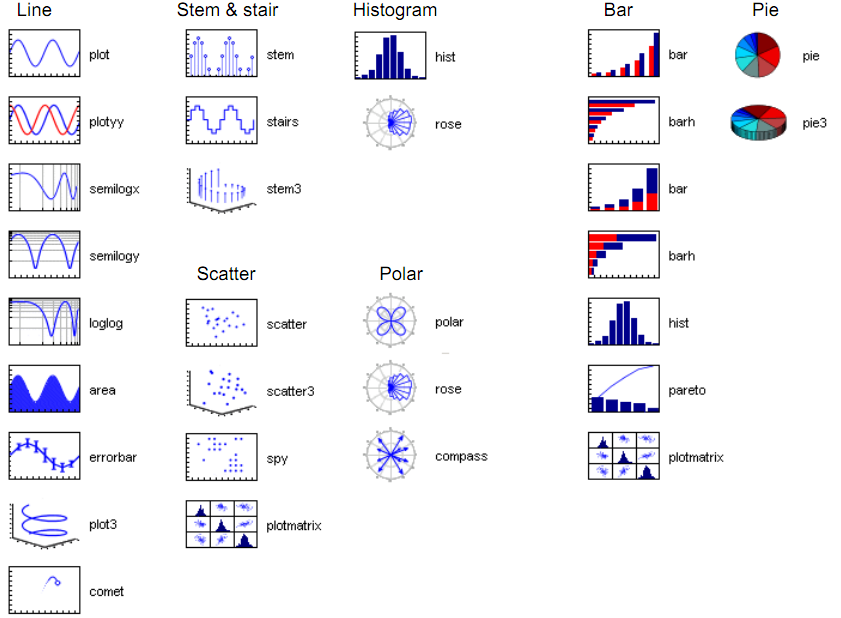
\includegraphics[width=450pt]{./Imagenes/graficos2d.png}
\end{center}

\section{Curvas en el plano}

Al construir la gráfica de una función $y=f(x)$ en el intervalo [a, b], se debe tener presente que \textbf{MATLAB} dibuja las curvas punto a punto; es decir, calcula los puntos $(x; f(x))$, para los valores de x que se le indique y representa dichos puntos unidos por un segmento. Por ello, se empieza estableciendo la matriz fila \textbf{x} cuyos elementos son los valores de \textbf{x} para los que se calculará el valor correspondiente de \textbf{f(x)}.

Para crear otros gráficos bi-dimensionales también se usa l comando \textbf{plot(x,y)}, donde los argumentos \textbf{x} e \textbf{y} son vectores con el mismo número de elementos.

Para representar una función del tipo $y=f(x)$ con el comando \textbf{plot}, el usuario necesita crear primero un vector con los valores de \textbf{x} del dominio de la función. En seguida, crear el vector $y=f(x)$ con los correspondientes valores de $f(x)$ y finalmente graficar la función $f$ con plot.

En el espacio de tres dimensiones la forma más sencilla de crear un gráfico 3D es mediante la 
función \textbf{plot3}, cuya sintaxis es bastante similar a la de la función \textbf{plot}. El comando \textbf{x=linspace(a,b,n)} crea el vector \textbf{x} de \textbf{n} elementos en el cual el primer elemento es \textbf{a} y el último es \textbf{b}, todos igualmente espaciados.

En \textbf{MATLAB} se usa el signo $\div$ para escribir los comentarios. Toda expresión después del signo $\div$ es ignorado por \textbf{MATLAB}. También usaremos los comandos \textbf{subplot}, \textbf{contour}, \textbf{contour3}, \textbf{quiver}, \textbf{comet}, etc.

Empezamos graficando funciones reales continuas definidas en un intervalo. Si $f$ es una función real de variable real, su gráfica es el conjunto $G(f)={(x;y)/y=f(x), x \in Dom(f)}$. Para comenzar vamos a estudiar en profundidad el comando \textbf{plot}, vamos ver algunos ejemplos con este comando y finalmente vamos a usar otros comandos que también sirven para representar curvas en el plano.

\section{El comando plot}

Los comandos de \textbf{MATLAB} cuentan con varios niveles de manipulación, y este es el caso del comando \textbf{plot}, el cual será fundamental para esta parte del curso. Los niveles iniciales son simples y por lo tanto fáciles de aprender y utilizar. El acceso a niveles finos exige trabajar con argumentos nuevos, más instrucciones y el manejo de una sintaxis más complicada. Comenzaremos viendo los diferentes niveles de forma gradual.

\subsection{Primer nivel}
El primer comando que trataremos es plot. Es una instrucción muy versátil y la más indicada para dibujar gráficas de funciones y curvas en el plano. Su sintaxis básica es

\begin{lstlisting}[language=Matlab]
>> plot(x,y)
\end{lstlisting}

que dibuja el vector y versus el vector x. Más en concreto une los puntos $(x_{i}, y_{i})$ mediante segmentos. Tomando un número suficientemente elevado de puntos trazamos con ello una gráfica suave, sin esquinas visibles.

Al ejecutar este comando se abre una ventana, \textbf{figure} en el vocabulario de \textbf{MATLAB}, donde se traza la correspondiente figura. Si \textbf{y} es real, \textbf{plot(y)} toma x=1:n donde n es la longitud de \textbf{y}. Si, por otro lado, y es un vector de números complejos, dibuja la parte imaginaria versus la parte real. Es decir, es equivalente a \textbf{plot(real(y),imag(y))}.

Las siguientes instrucciones utilizan el operador ":" (dos puntos) para crear un vector de los valores de \textbf{x} variando desde cero hasta 2 $\pi$ , para calcular el seno de estos valores y graficar el resultado.

\begin{lstlisting}[language=Matlab]
>> x = 0: pi/100 : 2*pi; 
>> y = sin(x); 
>> plot(x,y)
\end{lstlisting}

\begin{center}
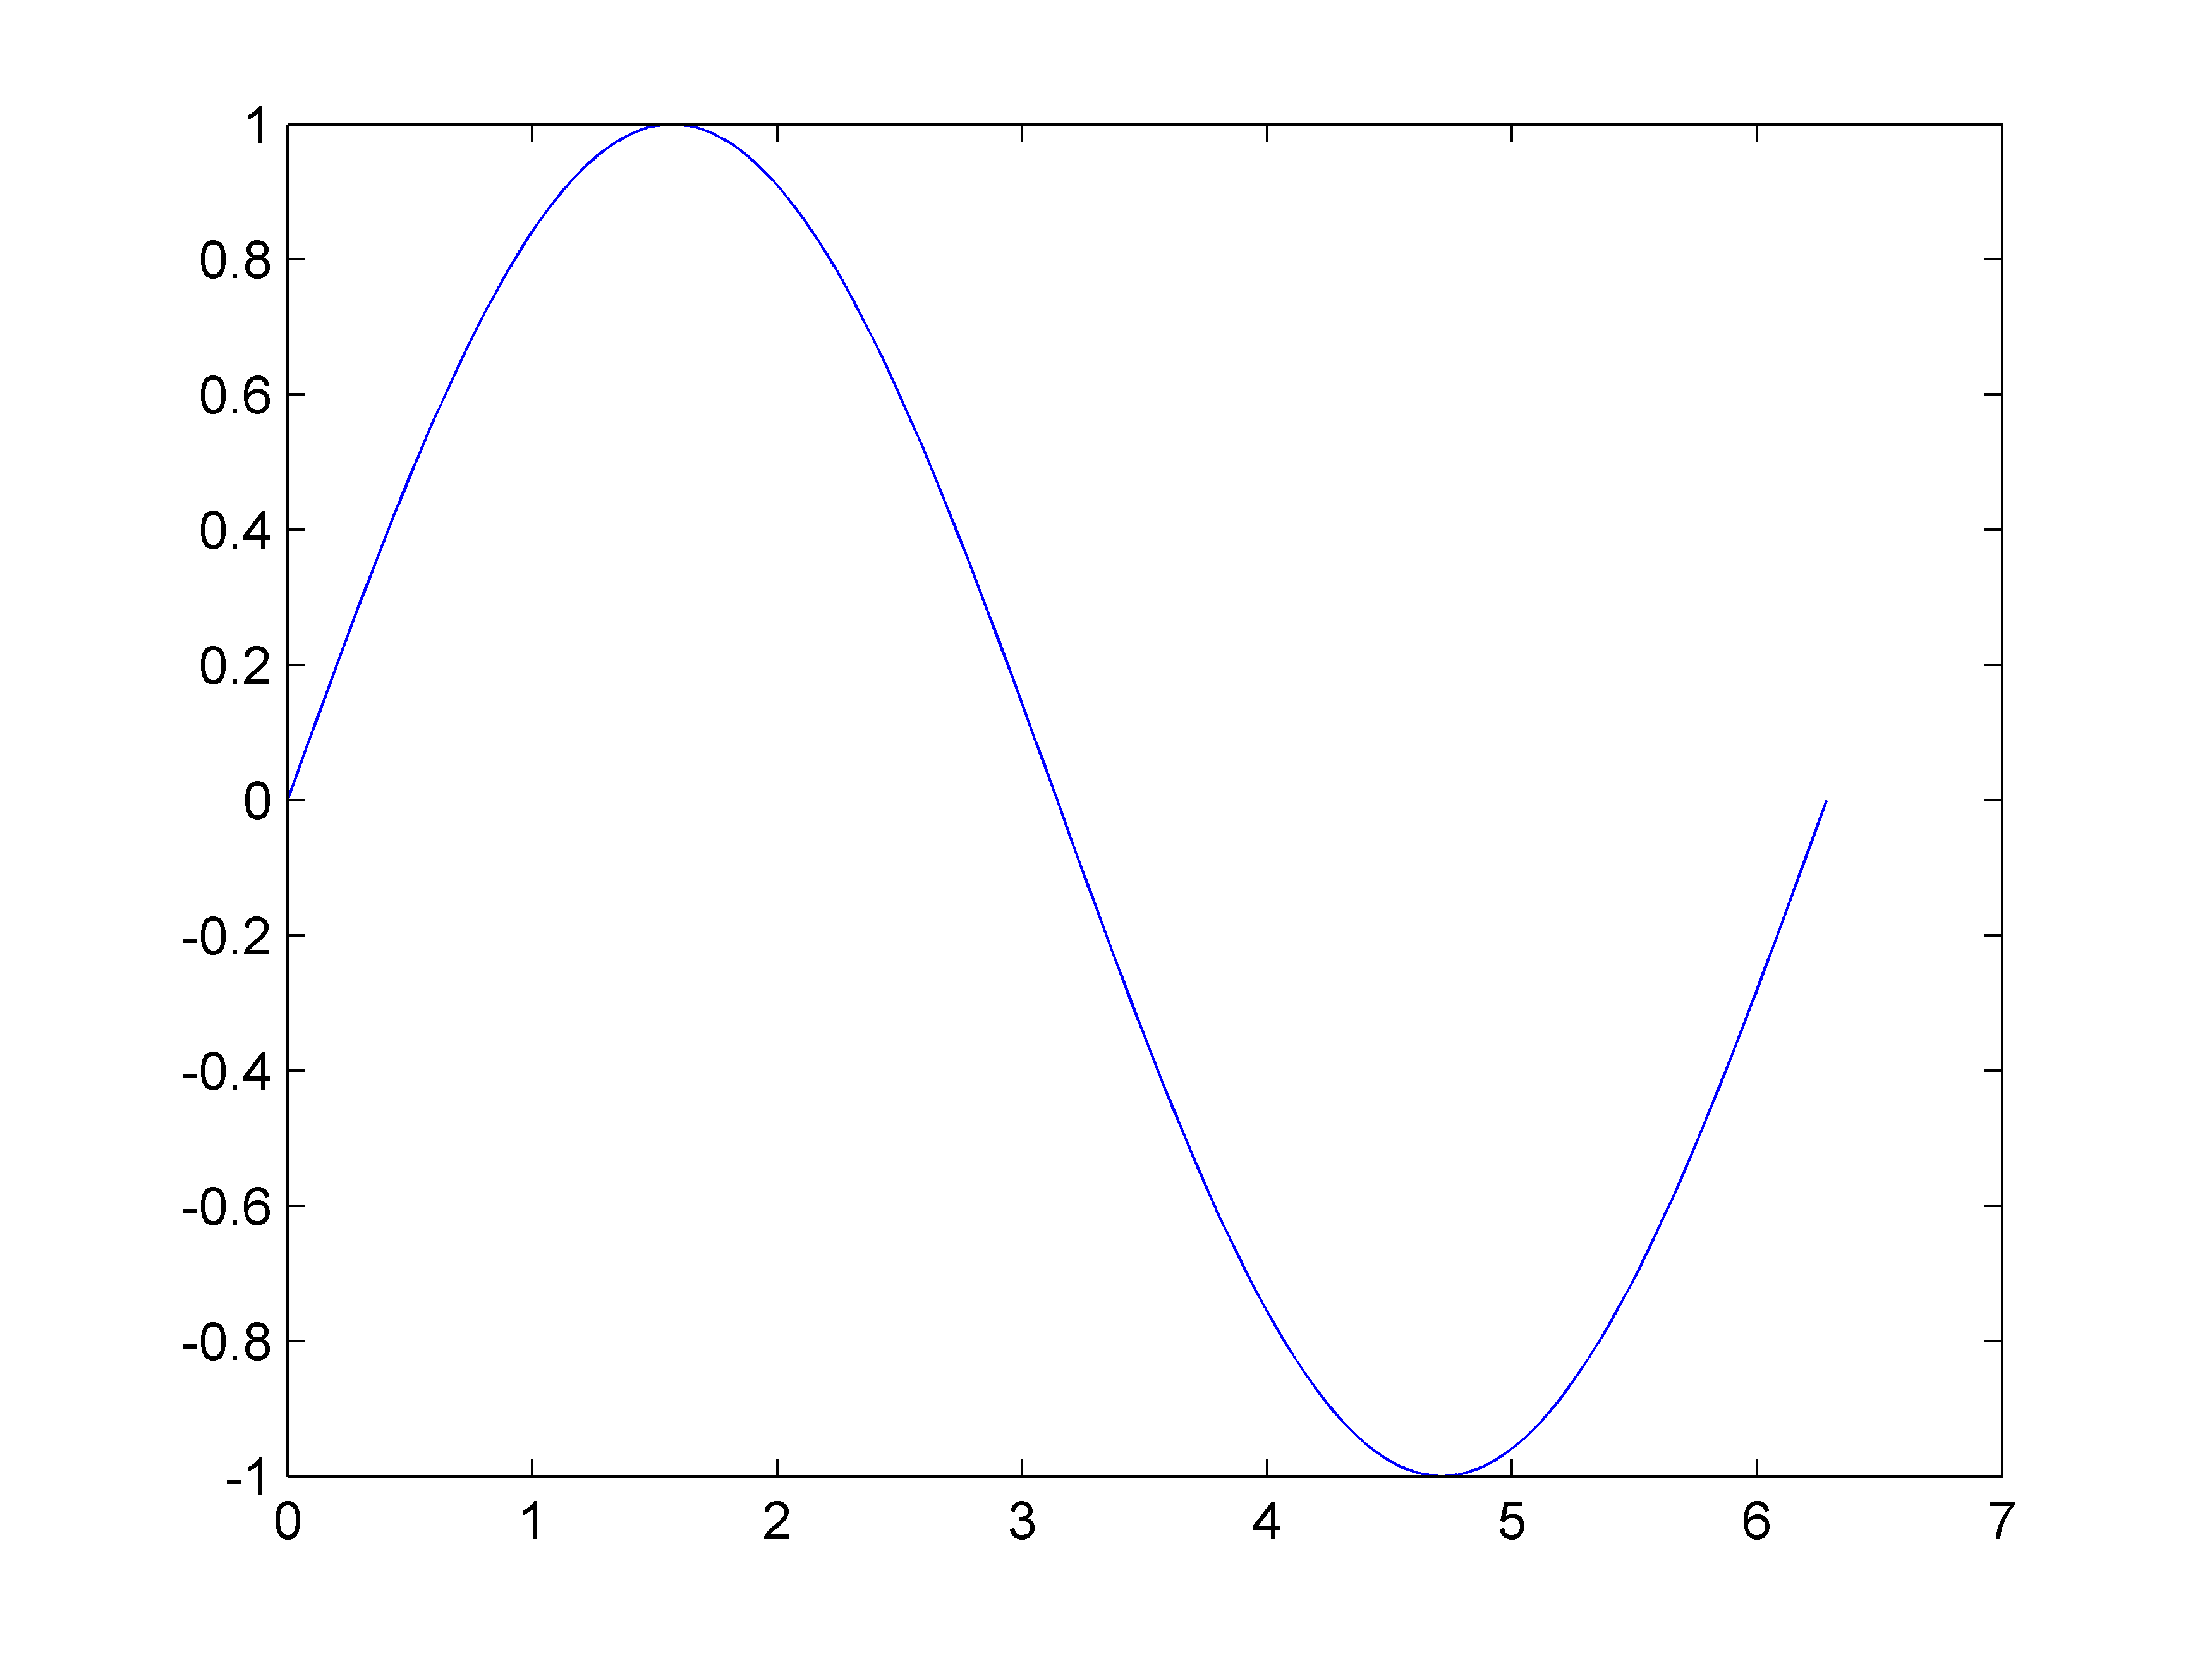
\includegraphics[width=300pt]{./Imagenes/seno1.png}
\end{center}

\subsubsection{Varias graficas en la misma imagen}

Múltiples pares de vectores x-y crean múltiples gráficos con una simple llamada a la sentencia 
plot. \textbf{MATLAB} les asigna automáticamente a través de una lista de colores predefinida (pero configurable por el usuario) para permitir la discriminación entre cada conjunto de datos. Por ejemplo, estas instrucciones grafican tres funciones de x, cada una con un color separado que las distingue. El comando \textbf{legend} provee una forma clara de identificar los gráficos individuales. 


\begin{lstlisting}[language=Matlab]
>> x = 0: pi/100 : 2*pi; 
>> y = sin(x);
>> y2 = sin(x-.25); 
>> y3 = sin(x-.5); 
>> plot(x,y,x,y2,x,y3)
>> legend('sin(x)','sin(x-.25)','sin(x-.5)'
\end{lstlisting}
\begin{center}
\includegraphics[width=300pt]{./Imagenes/senovarios.png}
\end{center}


\subsection{Segundo nivel}

El comando además acepta una serie de argumentos que, entre otras cosas, permiten controlar el color, el tipo de marcas sobre los puntos $(x_{i}, y_{i})$ y el formato de las líneas que los unen. Así, en su aspecto más general,

\begin{lstlisting}[language=Matlab]
>> plot(x,y,S)
\end{lstlisting}

dibuja y versus x, con S una cadena de caracteres que se construye con la primera columna especifica el color utilizado, la segunda la marca sobre cada punto y la tercera el patrón que siguen las líneas utilizadas para unir los puntos.

\begin{center}
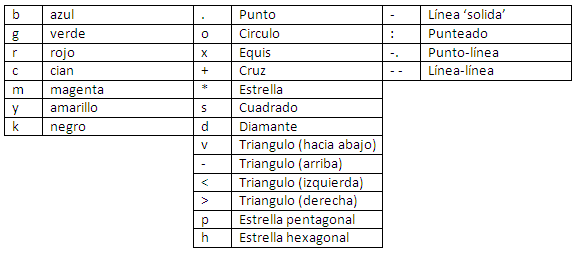
\includegraphics[width=300pt]{./Imagenes/comandosbasicos1.png}
\end{center}

La primer columna especifica el color utilizado, la segunda que tipo de marca se utilizara en cada punto y la tercer columna especifica el patrón que siguen las líneas utilizadas para unir los puntos.

\subsubsection{Líneas en gráficos}

En el caso de desearse una gráfica destinada a ser observada en blanco y negro, como por ejemplo  en fotocopias, conviene trazar líneas distintas en lugar de un tipo de línea y 
distintos colores. Por ejemplo, si la sentencia a usar es:

\begin{lstlisting}[language=Matlab]
>> x = 0: pi/100 : 2*pi; 
>> y = sin(x) 
>> y2 = sin(x-0.25) 
>> y3 = sin(x-0.5) 
>> plot (x,y,x,y2,':', x,y3,'--')
>> legend('sin(x)','sin(x-.25)','sin(x-.5)')
\end{lstlisting}
\begin{center}
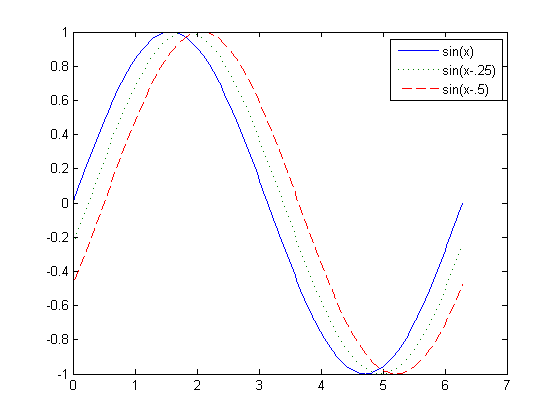
\includegraphics[width=300pt]{./Imagenes/senovariosmarca.png}
\end{center}

\subsubsection{Símbolos}

Si se especifica un tipo de símbolo pero no un estilo de línea, \textbf{MATLAB} exhibirá sólo el primero. Por ejemplo:

\begin{lstlisting}[language=Matlab]
>> clear 
>> x=0:0.02:2; 
>> y = 1 ./ ((x-.3).^2 + .01) + 1 ./ ((x-.9).^2 + .04) - 6; 
>> plot(x,y,'ks') 
\end{lstlisting}
\begin{center}
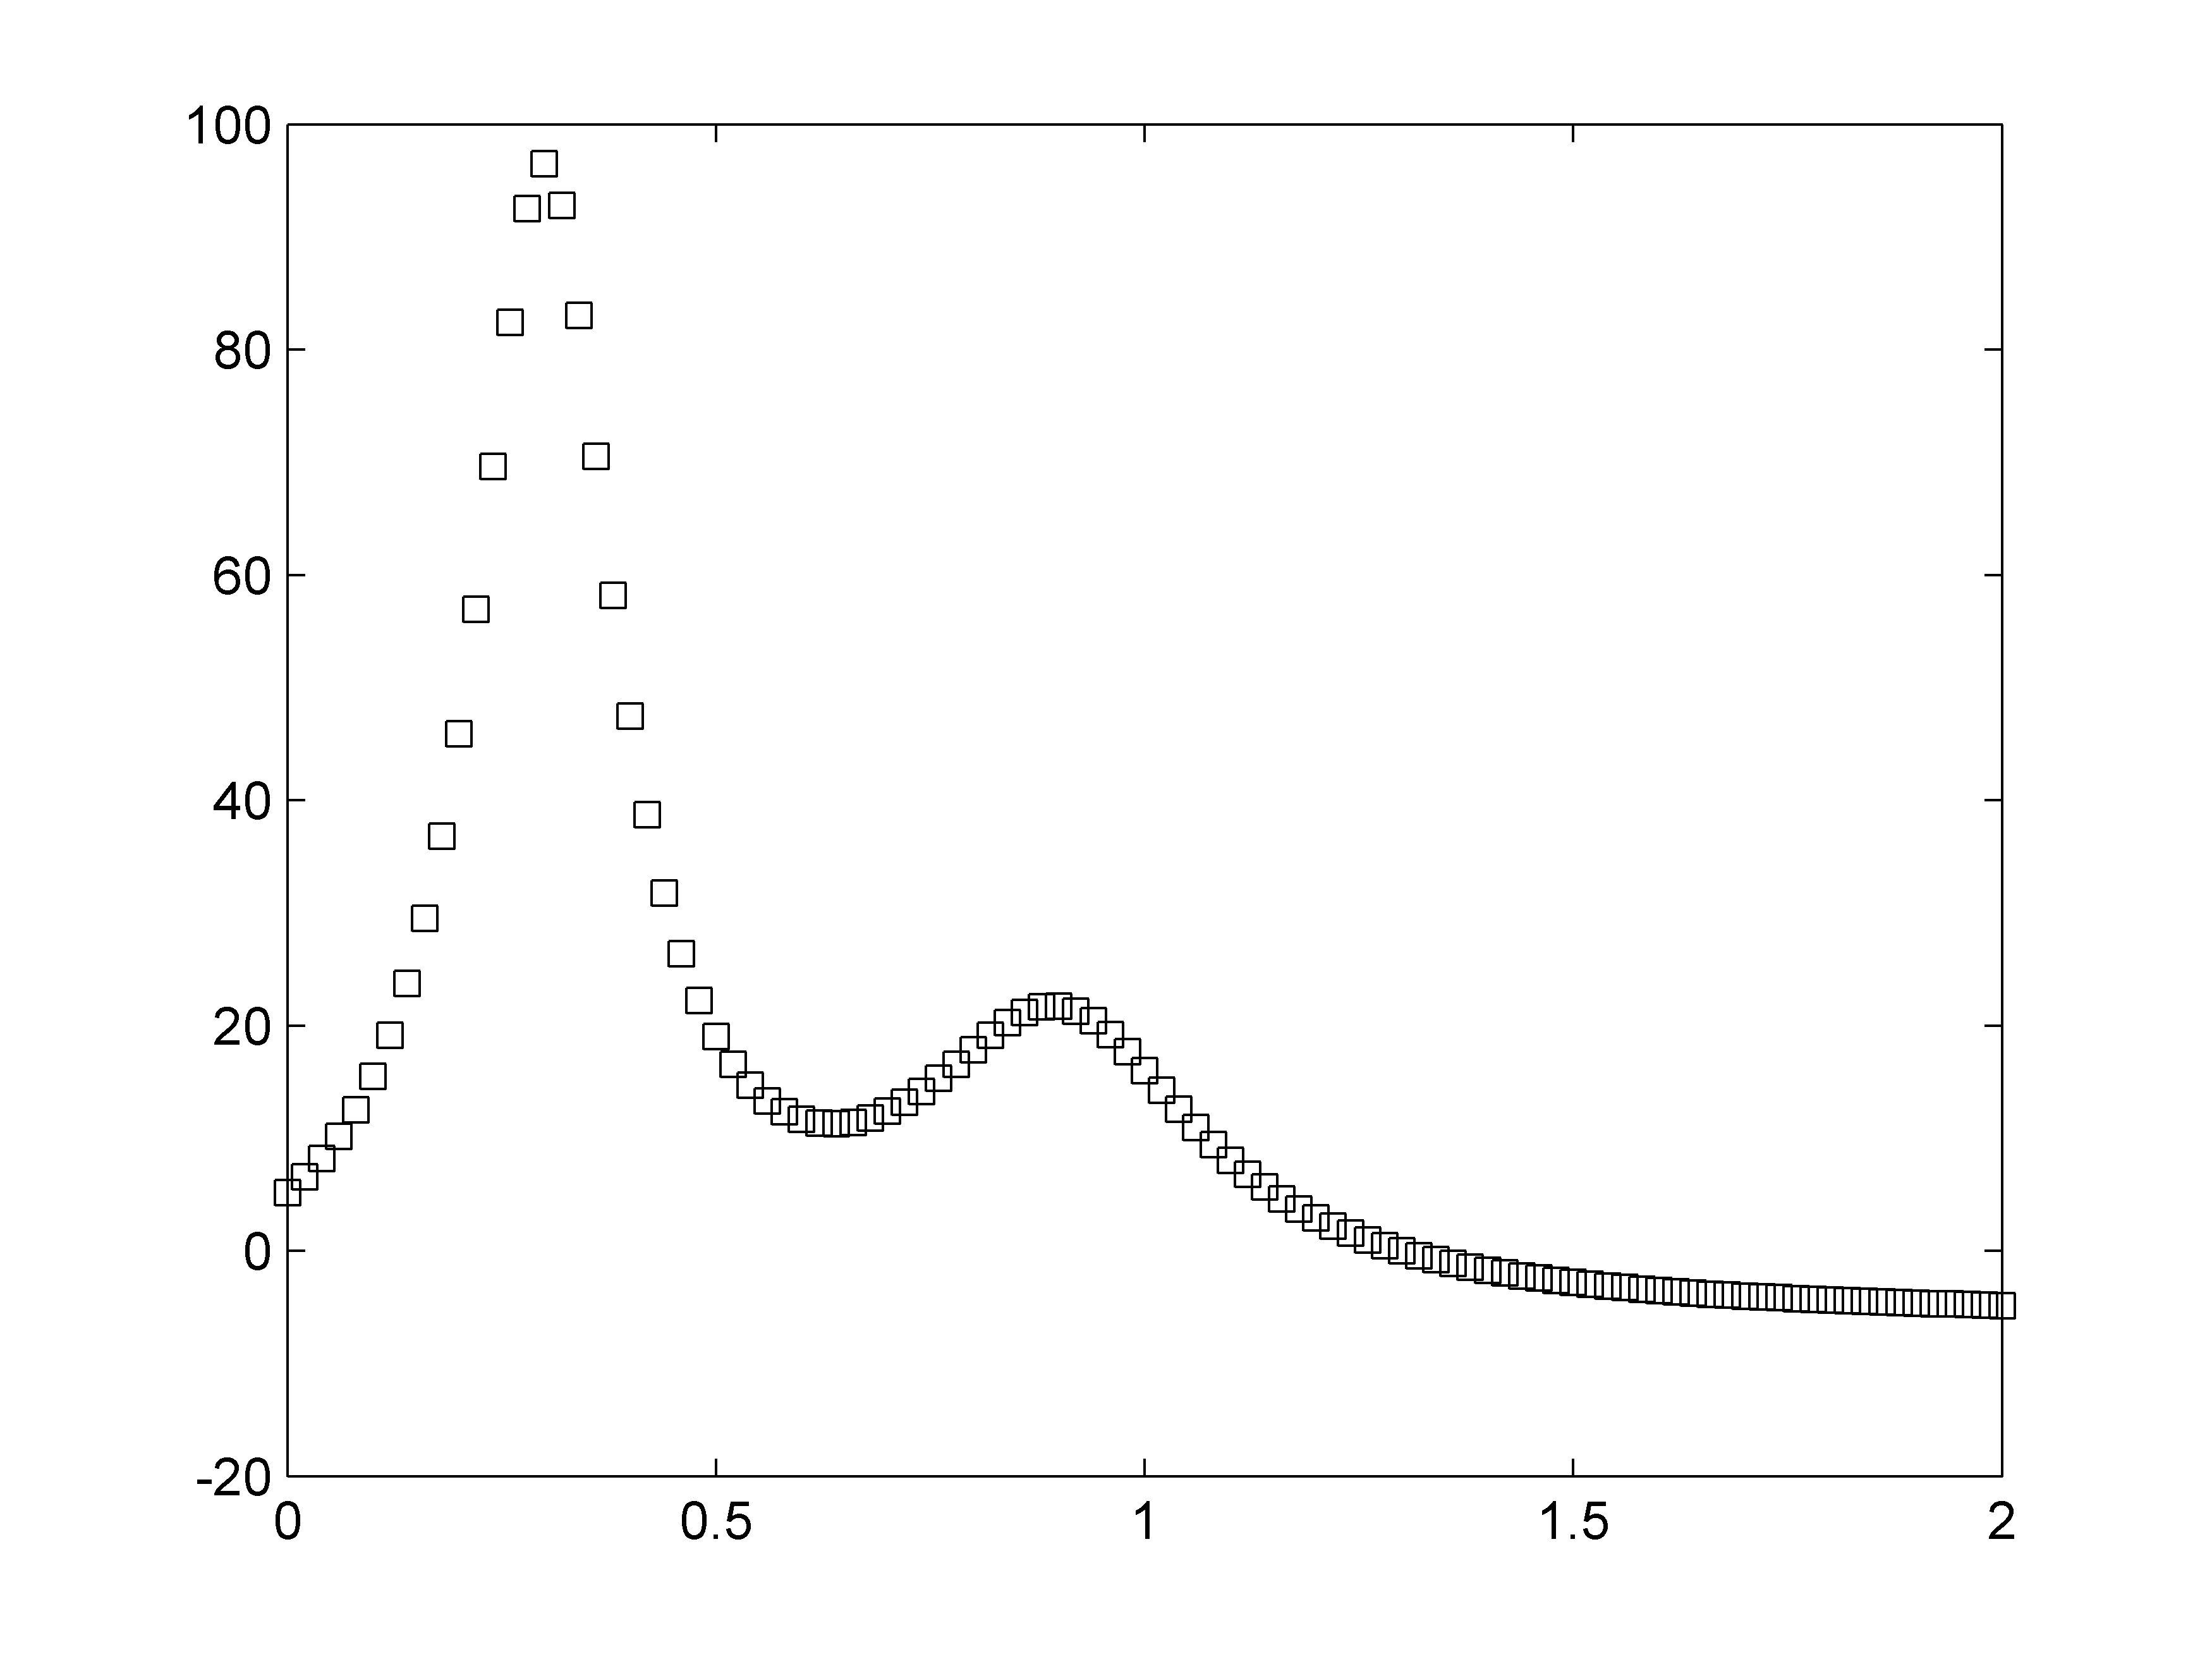
\includegraphics[width=300pt]{./Imagenes/simbolo1.png}
\end{center}

Si deseamos que aparezcan líneas con símbolos, se puede escribir, por ejemplo $plot(x,y,'r:+')$ 
que gráfica una línea roja de puntos y coloca marcadores de signo más en cada punto.:

\begin{lstlisting}[language=Matlab]
>> clear 
>> x=0:0.02:2; 
>> y = 1 ./ ((x-.3).^2 + .01) + 1 ./ ((x-.9).^2 + .04) - 6;
>> plot(x,y,'r:+')
\end{lstlisting}
\begin{center}
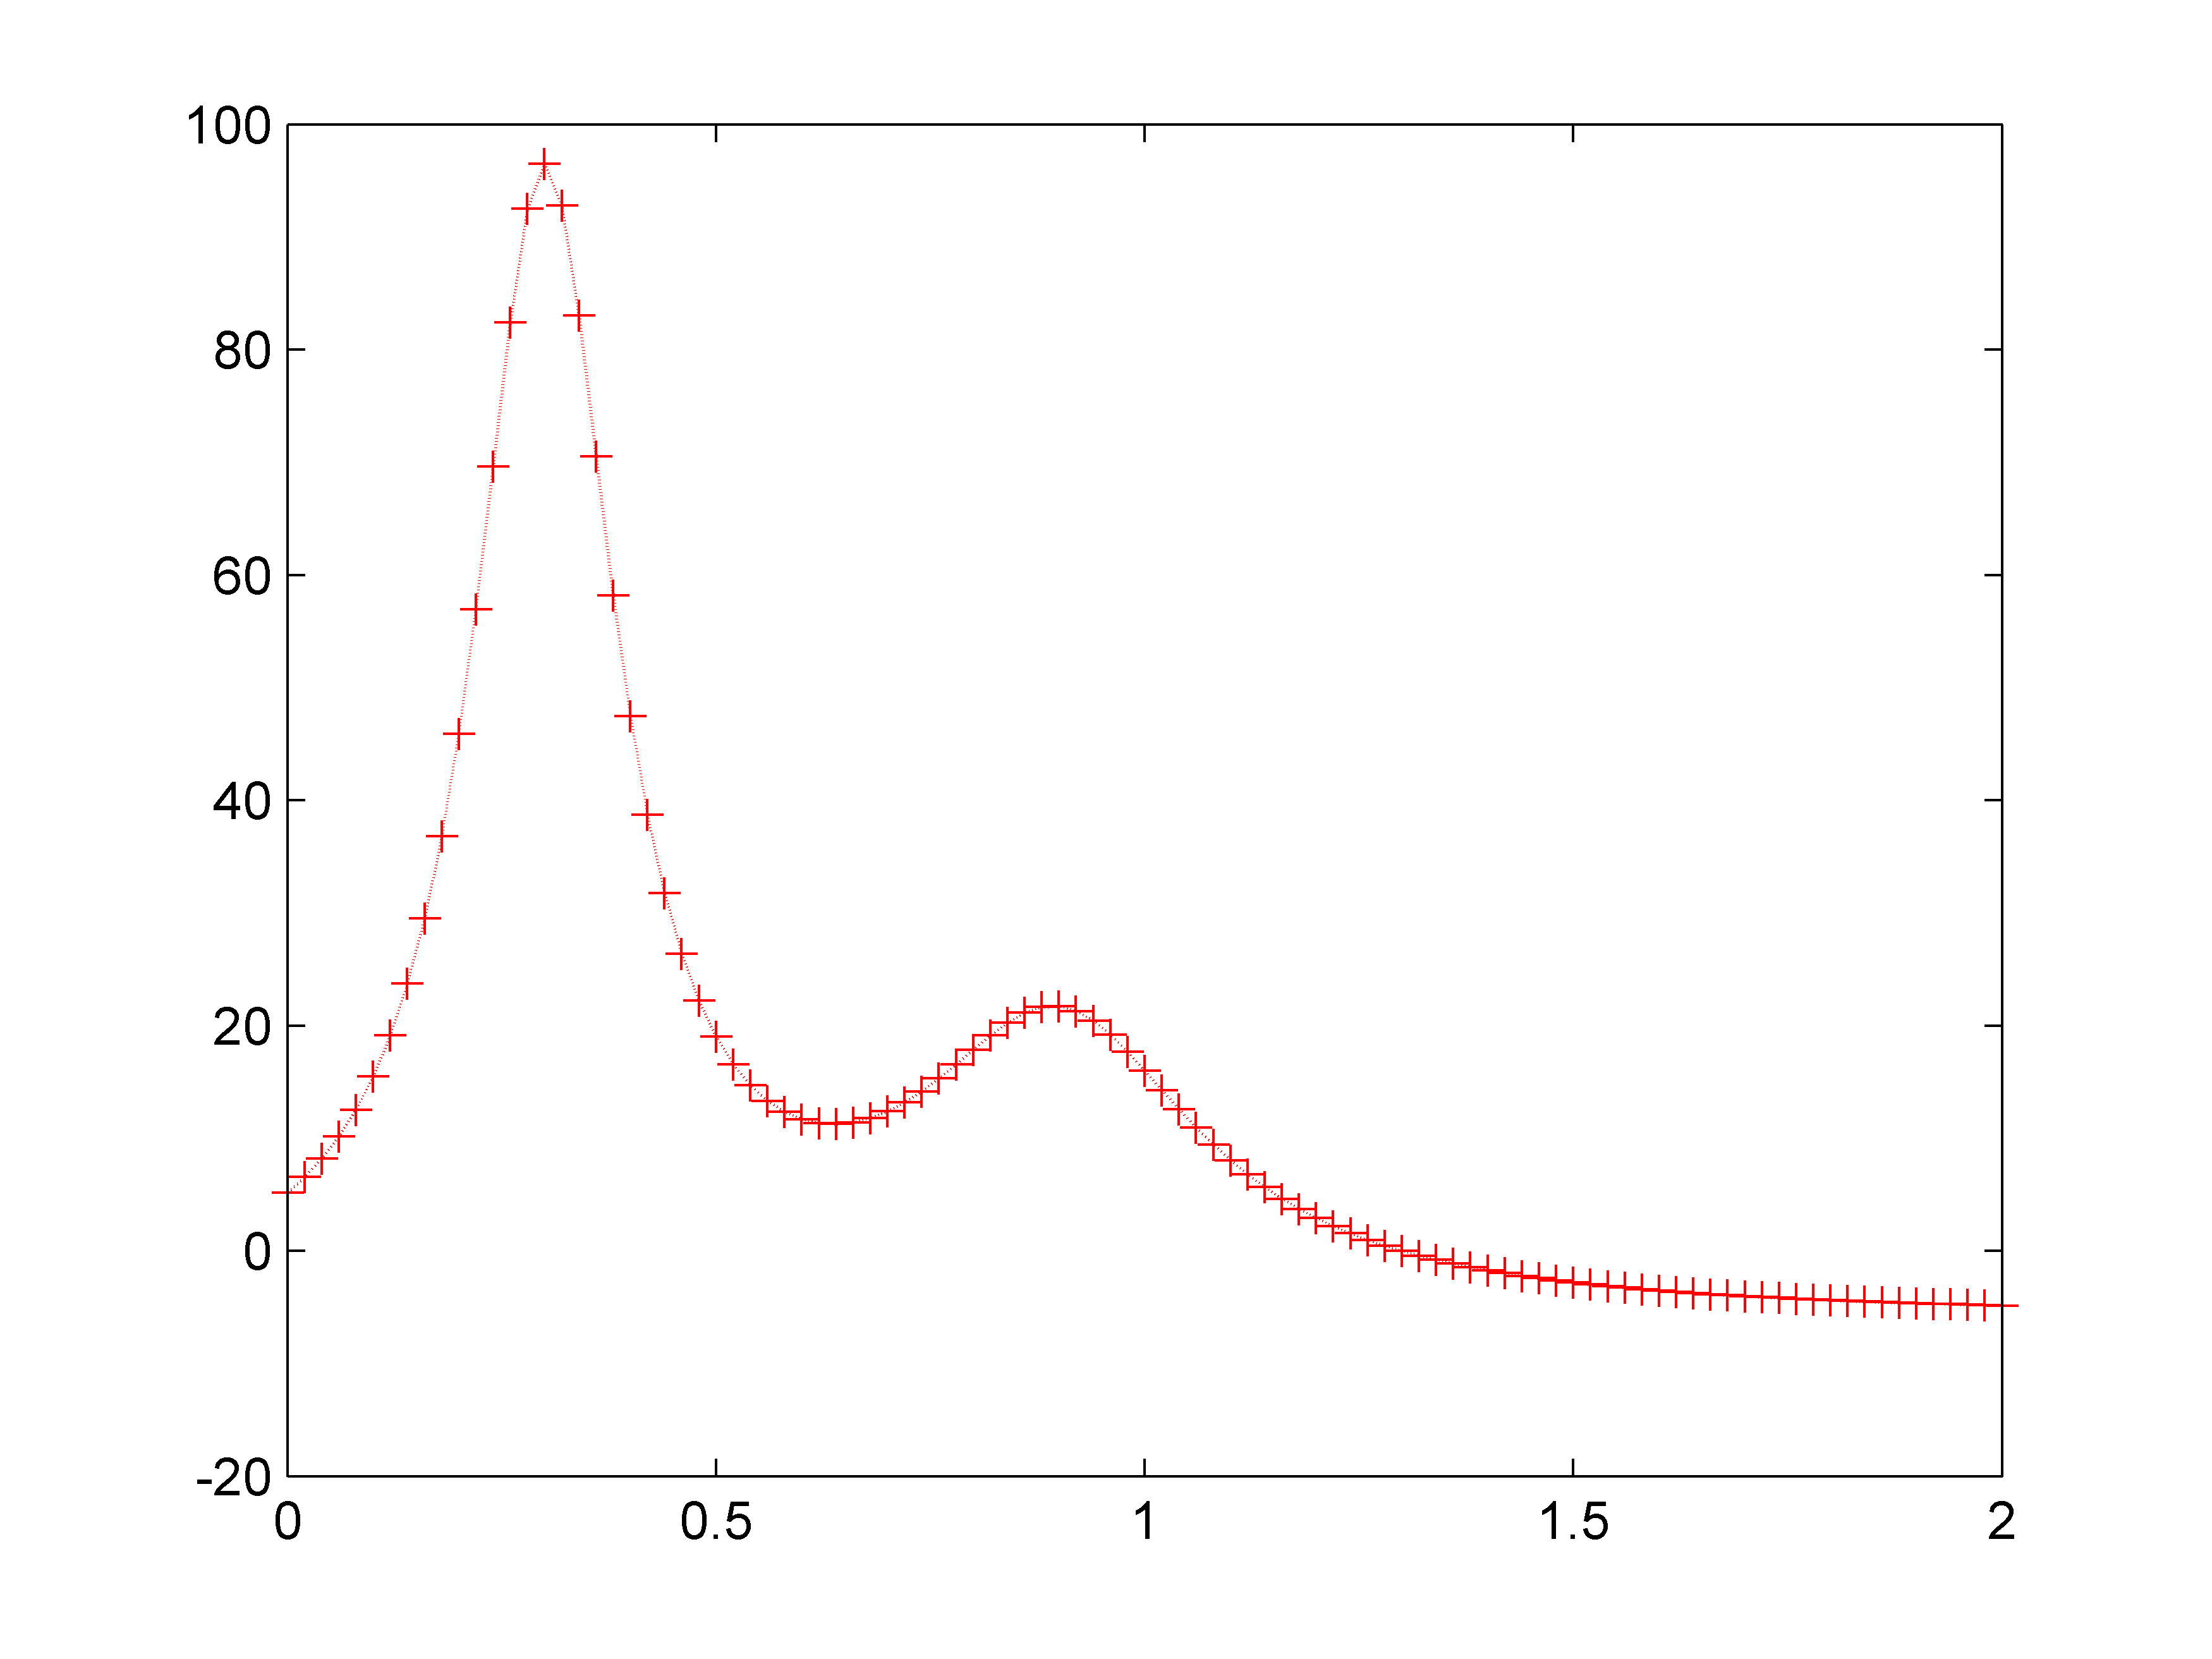
\includegraphics[width=300pt]{./Imagenes/simbolo2.png}
\end{center}

\subsubsection{Comandos hold on y hold off}

Normalmente, si se ejecuta una sentencia \textbf{plot}, y luego otra, en el curso de una sesión o 
programa, la ultima es la única que puede verse pues cada sentencia plot borra las anteriores. 
Por ejemplo:

\begin{lstlisting}[language=Matlab]
>> alfa = 0:0.02:2*pi; 
>> y = sin(alfa); 
>> plot (alfa,y) 
>> z = cos(alfa) 
>> plot(alfa,z)
\end{lstlisting}
 
permitiría visualizar sólo el gráfico del coseno, pero no el del seno. Una opción sería, como ya se vio, graficar conjuntamente las dos funciones, pero por distintas razones, surge a veces la necesidad de realizar una construcción secuencial de un gráfico para adicionar curvas 
gradualmente.  Esto se puede hacer mediante el uso de la sentencia \textbf{hold on} (sostener o mantener activo).

\begin{lstlisting}[language=Matlab]
>> x=0:0.02:2*pi; 
>> y = sin(x) 
>> plot(x,y) 
>> hold on 
>> z = cos(x) 
>> plot(x,z,':') 
>> hold off
\end{lstlisting}
\begin{center}
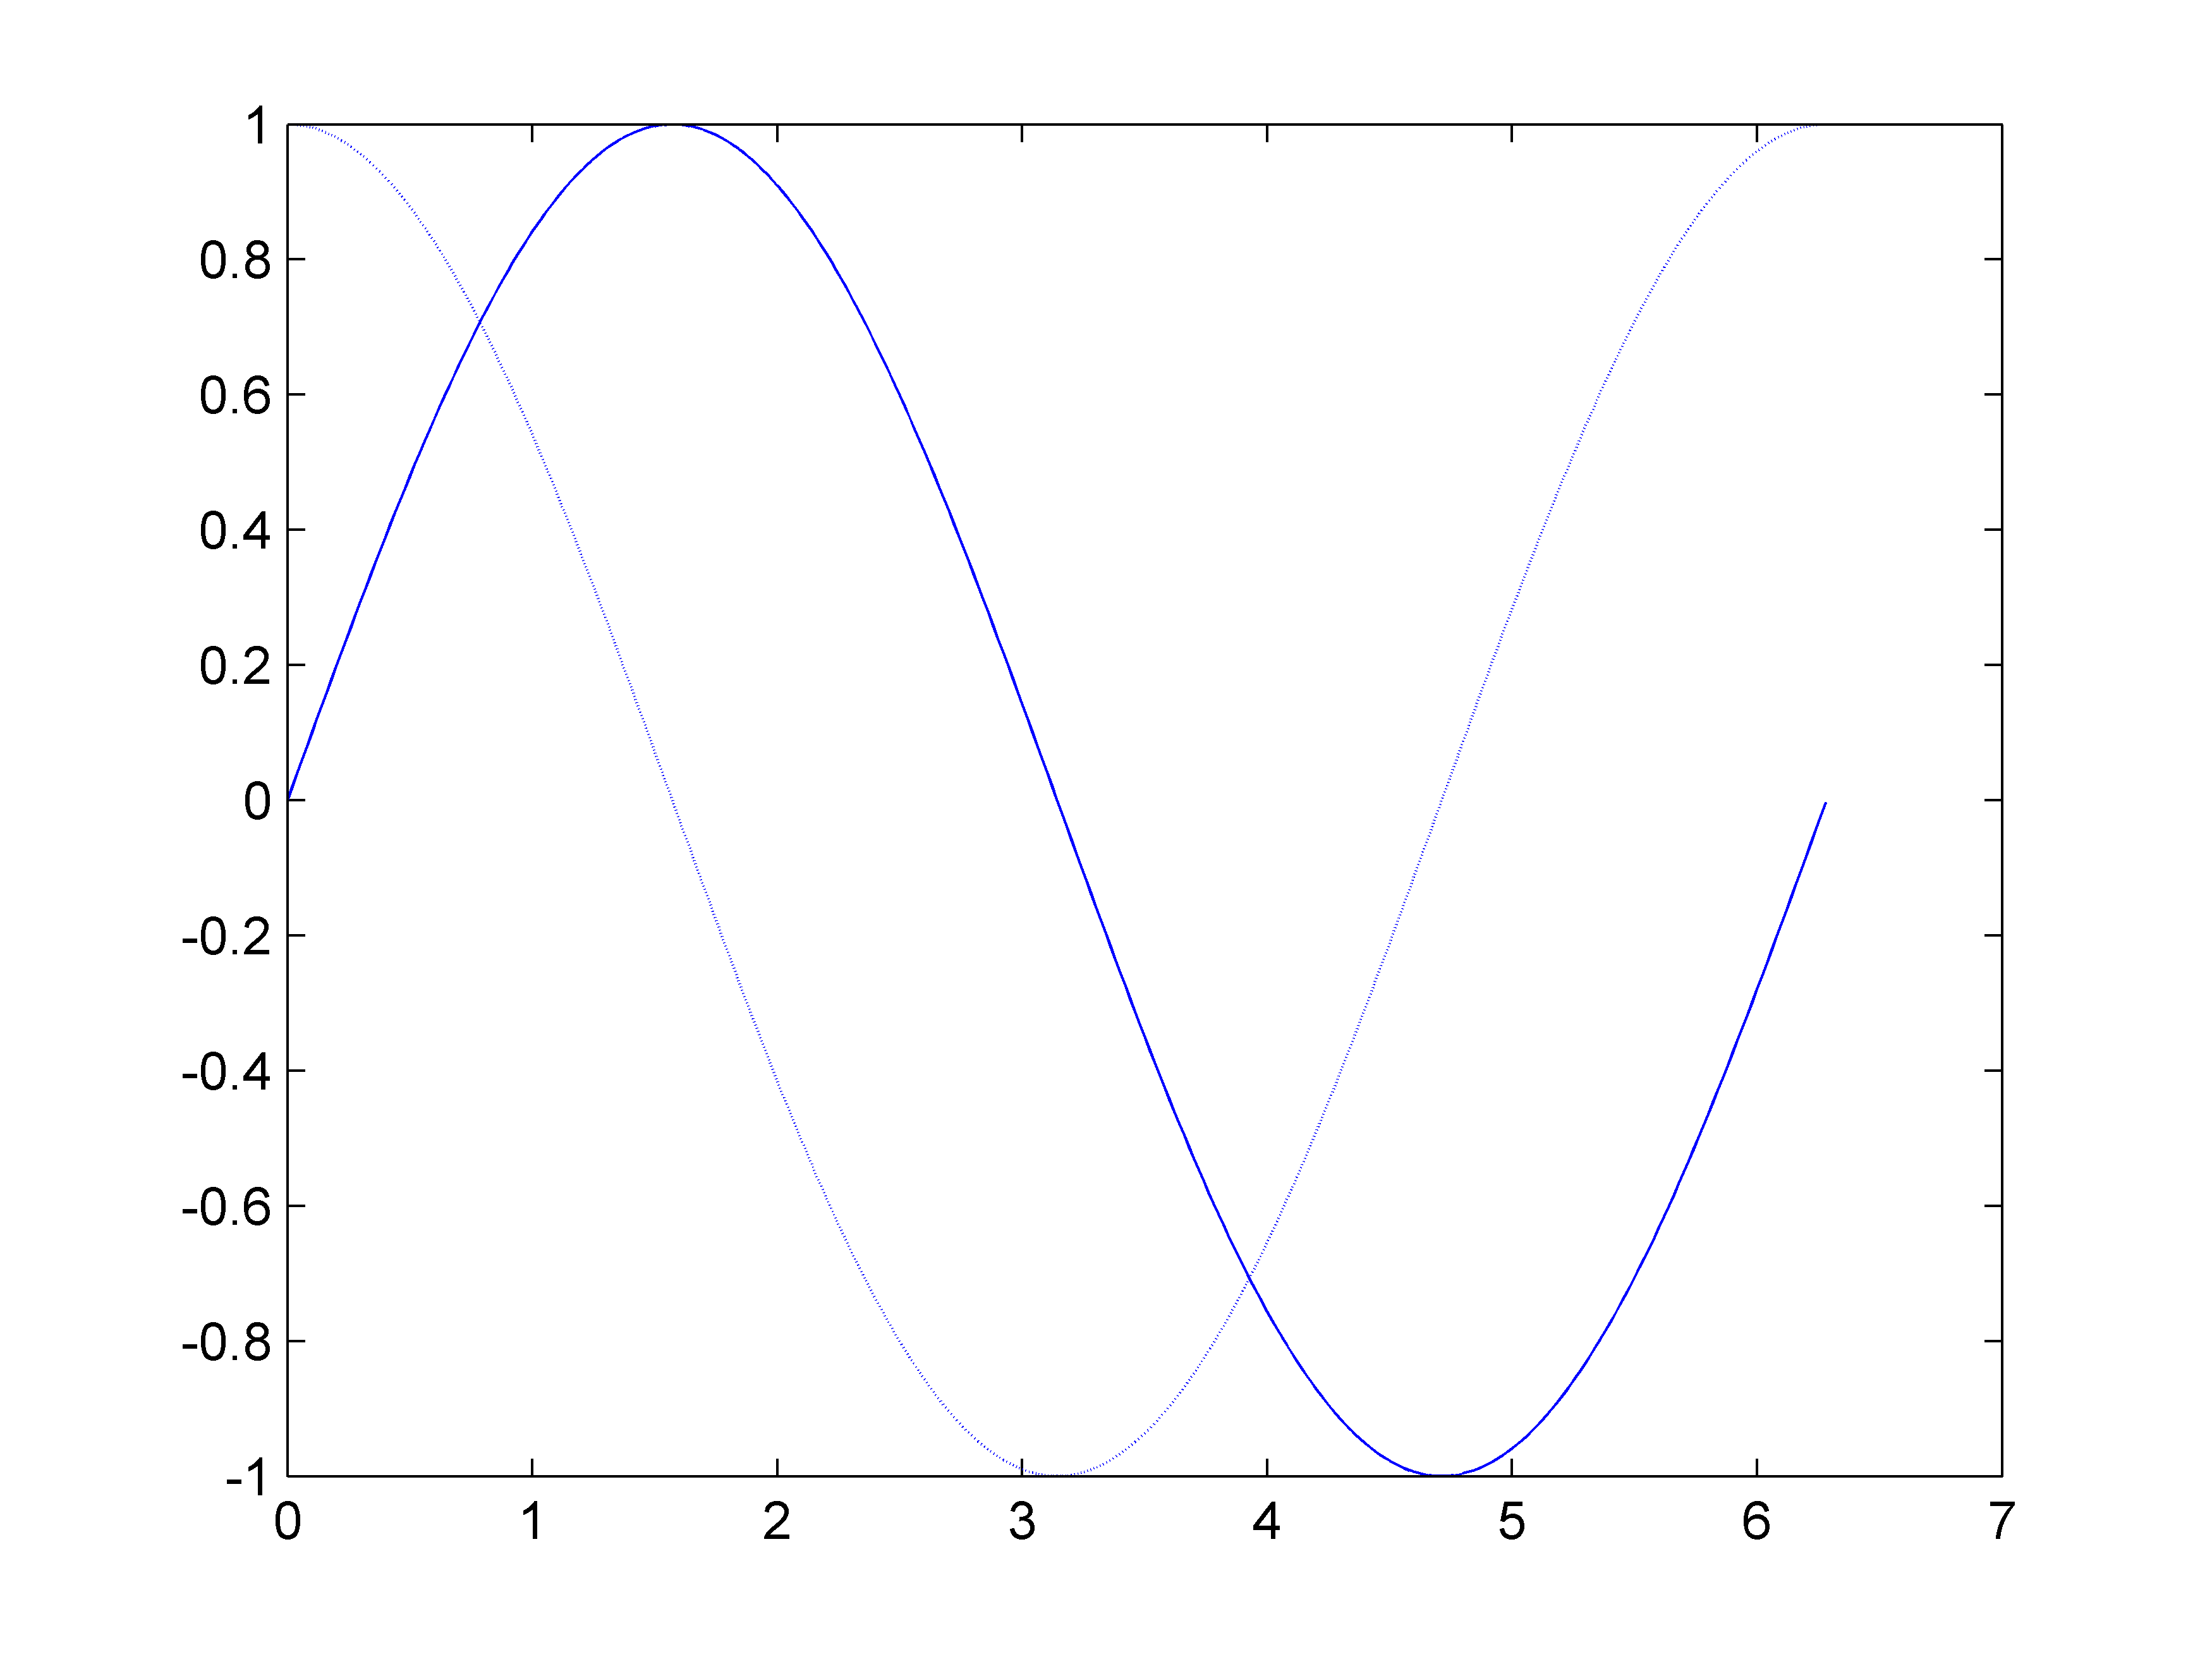
\includegraphics[width=300pt]{./Imagenes/holdon.png}
\end{center}

\subsubsection{Comando figure}

El comando \textbf{figure} permite mantener simultáneamente varias figuras para su observación, lo que resulta sumamente útil para evaluar los resultados de un programa. Por ejemplo:

\begin{lstlisting}[language=Matlab]
>> x = 0:0.02:2*pi; 
>> y = cos(x) 
>> z = exp(-x).*cos(x); 
>> plot(x,y) 
>> figure(2) 
>> plot(x,z) 
\end{lstlisting}

\subsubsection{Subdivisión de la ventana de gráficos}

A efectos de exhibir simultáneamente varias figuras sin solapamientos, se puede subdividir la 
ventana gráfica con la función subplot() en m particiones horizontales y n verticales. Cada una de esas particiones se puede llamar sub-gráfico. El subíndice \textit{i} identifica la subdivisión que se convierte en activa.

\begin{lstlisting}[language=Matlab]
>> x=0:0.1:10;
>> subplot(2,1,1), plot(x,sin(x));
>> subplot (2,1,2), plot(x,log(x))
\end{lstlisting}
\begin{center}
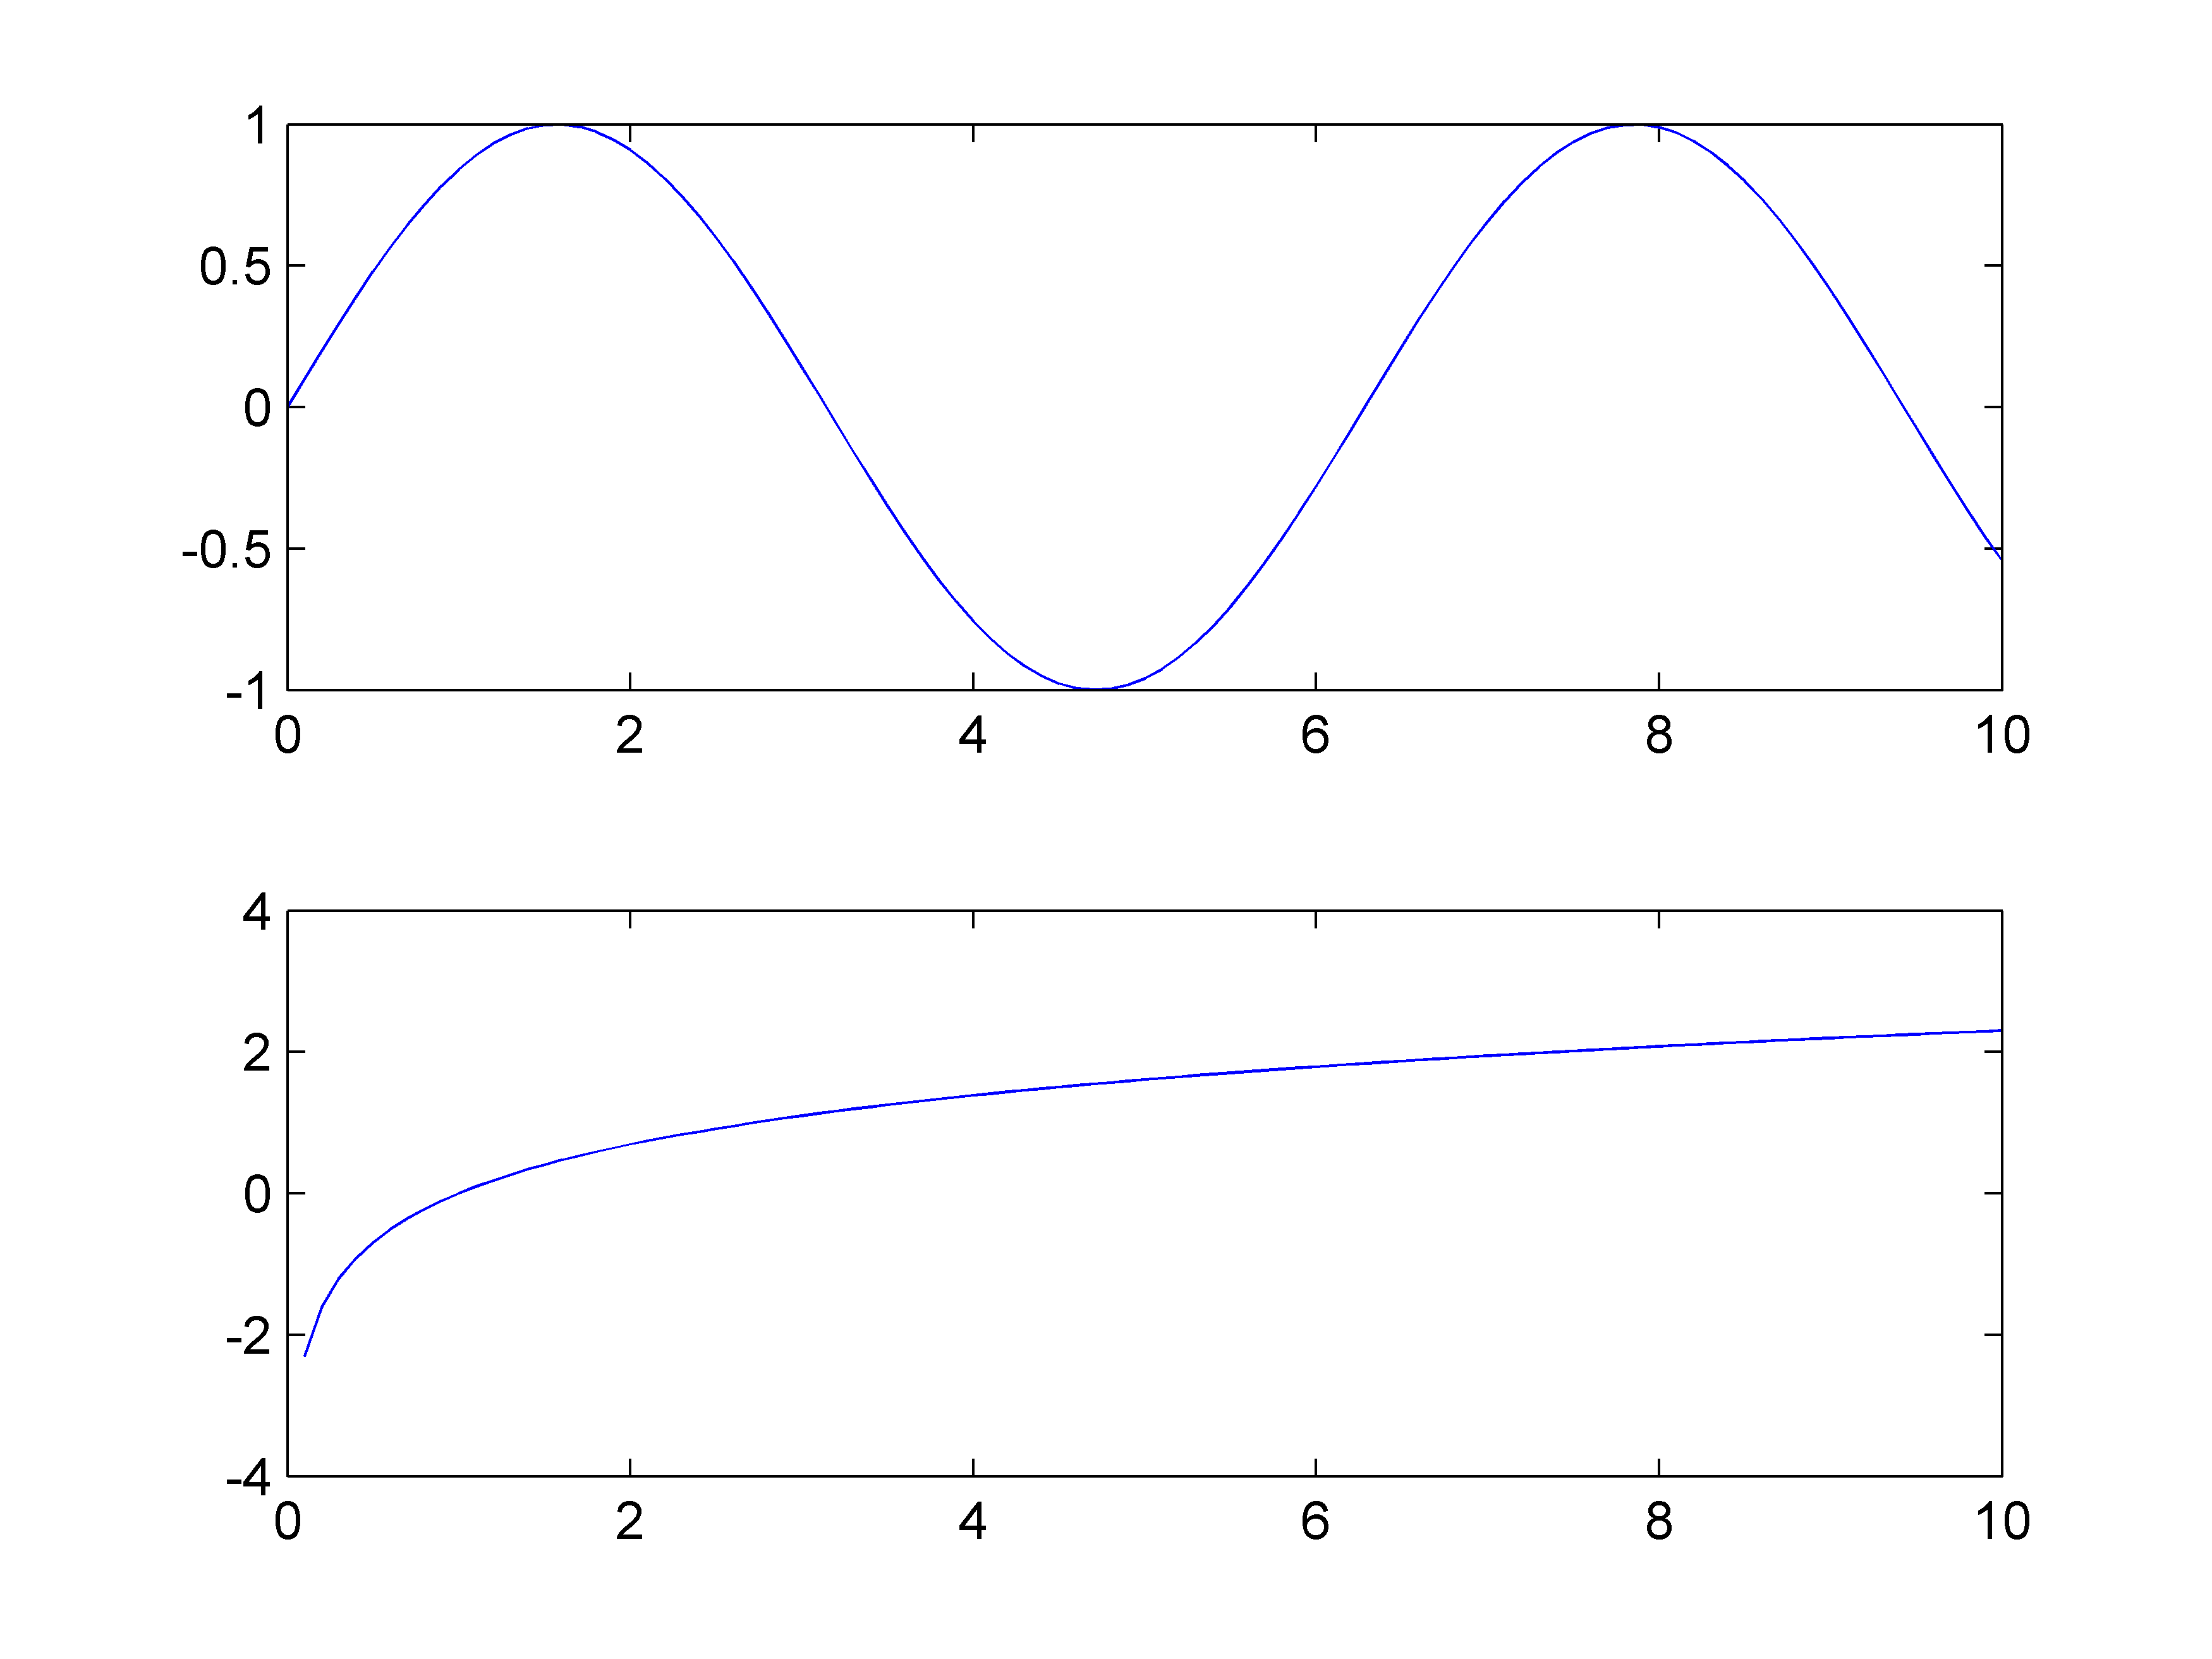
\includegraphics[width=300pt]{./Imagenes/subplot.png}
\end{center}

Ejemplo de subdivisión en dos filas y dos columnas:

\begin{lstlisting}[language=Matlab]
>> x=0: pi/25: 6*pi;  
>> y= cos(x); 
>> z= abs(cos(x))+1;  
>> w=exp(-0.2.*x).*y+ 2; 
>> v= exp(+0.2.*x).*y +2;  
>> subplot(2,2,1), plot(x,y); xlabel ('x', 'Fontsize', 18);ylabel('y','Fontsize', 18)  
>> subplot(2,2,2), plot(x,z); xlabel ('x', 'Fontsize', 18);ylabel('z', 'Fontsize', 18) 
>> subplot(2,2,3), plot(x,w);xlabel ('x', 'Fontsize', 18');ylabel('w','Fontsize', 18) 
>> subplot(2,2,4), plot(x,v); xlabel ('x', 'Fontsize', 18);ylabel('v', 'Fontsize', 18)
\end{lstlisting}
\begin{center}
\includegraphics[width=300pt]{./Imagenes/subplot2.png}
\end{center}


\subsection{Tercer nivel}

En este nivel se puede acceder a detalles concretos del gráfico como son el tamaño y el color de las marcas y el ancho de una linea entre otras cosas. Las diferentes opciones son:

\begin{itemize}
\item \textbf{color}: color de la linea.
\item \textbf{LineWidth}: ancho de una linea.
\item \textbf{Marker}: marca que se coloca en los puntos evaluados.
\item \textbf{MarkerEdgeColor}: color del borde de las marcas.
\item \textbf{MarkerFaceColor}: color de la marca.
\item \textbf{MarkerSize}: tamanio de la marca
\end{itemize}

Para especificar un color, se pueden utilizar los caracteres {b,g,r,c,m,y,k} o bien un vector con tres componentes con valores entre 0 y 1 que especifica un color según el estándar RGB. Un ejemplo del uso de estos comandos:

\begin{lstlisting}[language=Matlab]
>> x=0.01:0.2:2;
>> y=sin(x)./x;
>> plot(x,y,'o-.','color',[0.2 0.4 0.6],'linewidth',2,'markeredgecolor',...
'k','markerfacecolor',[0.9 0.6 0.4],'markersize',9)
\end{lstlisting}
\begin{center}
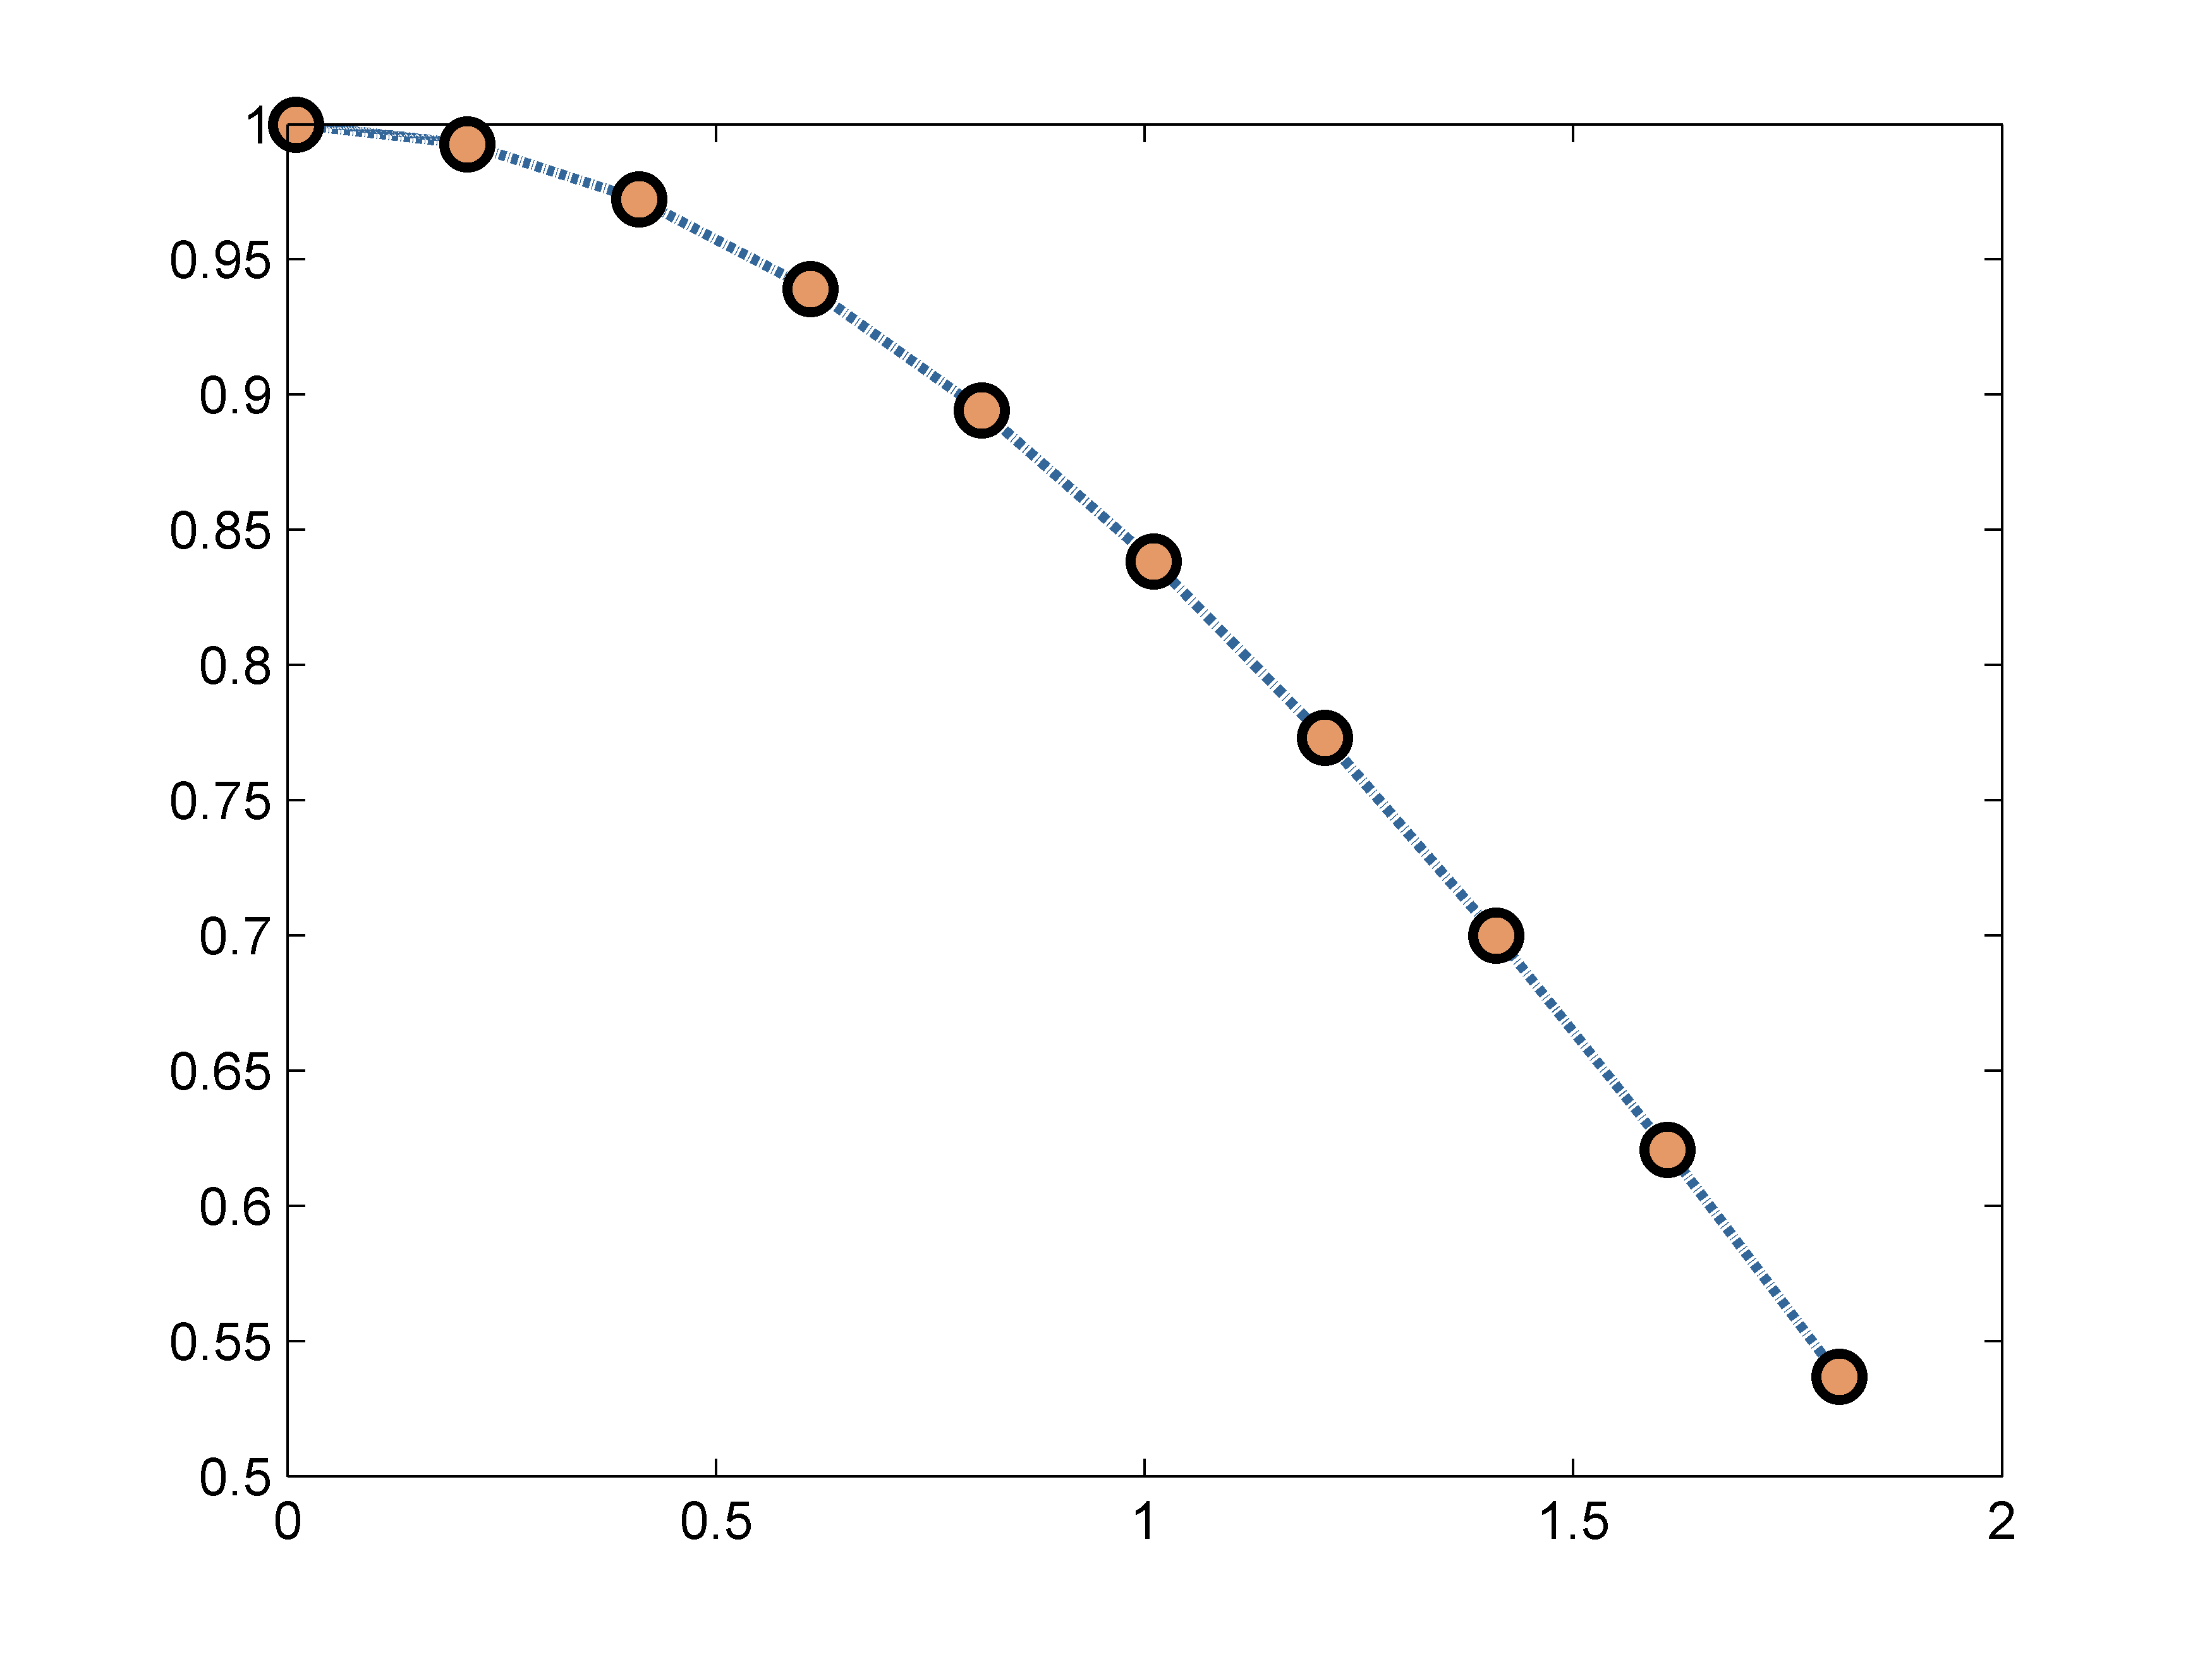
\includegraphics[width=300pt]{./Imagenes/tercernivel.png}
\end{center}

\section{Comandos asociados a plot}

Hay comandos que nos permiten controlar la ventana donde se mostraran los gráficos. Entre los más usados están:

\begin{itemize}
\item \textbf{clf}: borra la ventana actual (figure) de gráficos.
\item \textbf{cla}: borra los ejes.
\item \textbf{hold}: nos permite solapar varias gráficas en una misma ventana.
\item \textbf{axis}: puede controlar los ejes X e Y.
\item \textbf{xlim,ylim}: especifica los limites del dibujo. Se pueden utilizar para centrarlo.
\item \textbf{grid}: grid on muestra una malla en pantalla, y grid off la borra.
\item \textbf{legend}: despliega una leyenda, esto es, un cuadro detallando las gráficas.
\item \textbf{text}: ingresar un texto
\item \textbf{xlabel,ylabel}: etiqueta los ejes X e Y.
\item \textbf{title}: coloca un titulo en la cabecera del dibujo.
\item \textbf{whitebg}: asigna un color al fondo de la figura.
\end{itemize}

A continuación vamos a ver un ejemplo donde representamos 4 funciones, y usamos varios de los comandos antes mencionados para tratar los datos de la ventana y de los gráficos en si:

\begin{lstlisting}[language=Matlab]
>> figure(1) % desplegamos ventana 1
>> clf % borramos todo
>> x=linspace(0,5,100);
>> f=inline('exp(-n*x).*cos(x)','n','x'); % funciones vectorizadas
>> hold on % solapamiento de graficas
>> y=f(1/3,x);
>> plot(x,y,'k--','linewidth',2)
>> y=f(1,x);
>> plot(x,y,'r-.','linewidth',2)
>> y=f(3,x);
>> plot(x,y,':','color',[0.0,0.0,0.5],'linewidth',2)
>> y=f(9,x);
>> plot(x,y,'-','color',[0.0,0.3,0.0],'linewidth',2)
>> grid on % desplegamos la red
>> xlim([-0.5,6]), ylim([-0.25,0.5]) % rango de los graficos
>> xlabel('Eje X','fontname', 'Comic Sans Ms', 'fontsize',12)
>> ylabel('Eje Y','fontname', 'Comic Sans Ms', 'fontsize',12)
>> title('Graficas de ejemplo','fontsize',16,'fontname','Times new roman')
>> legend('exp(-x/3).*cos(x)', 'exp(-x).*cos(x)','exp(-3x)*cos(x)', 'exp(-9x).*cos(x)');
\end{lstlisting}
\begin{center}
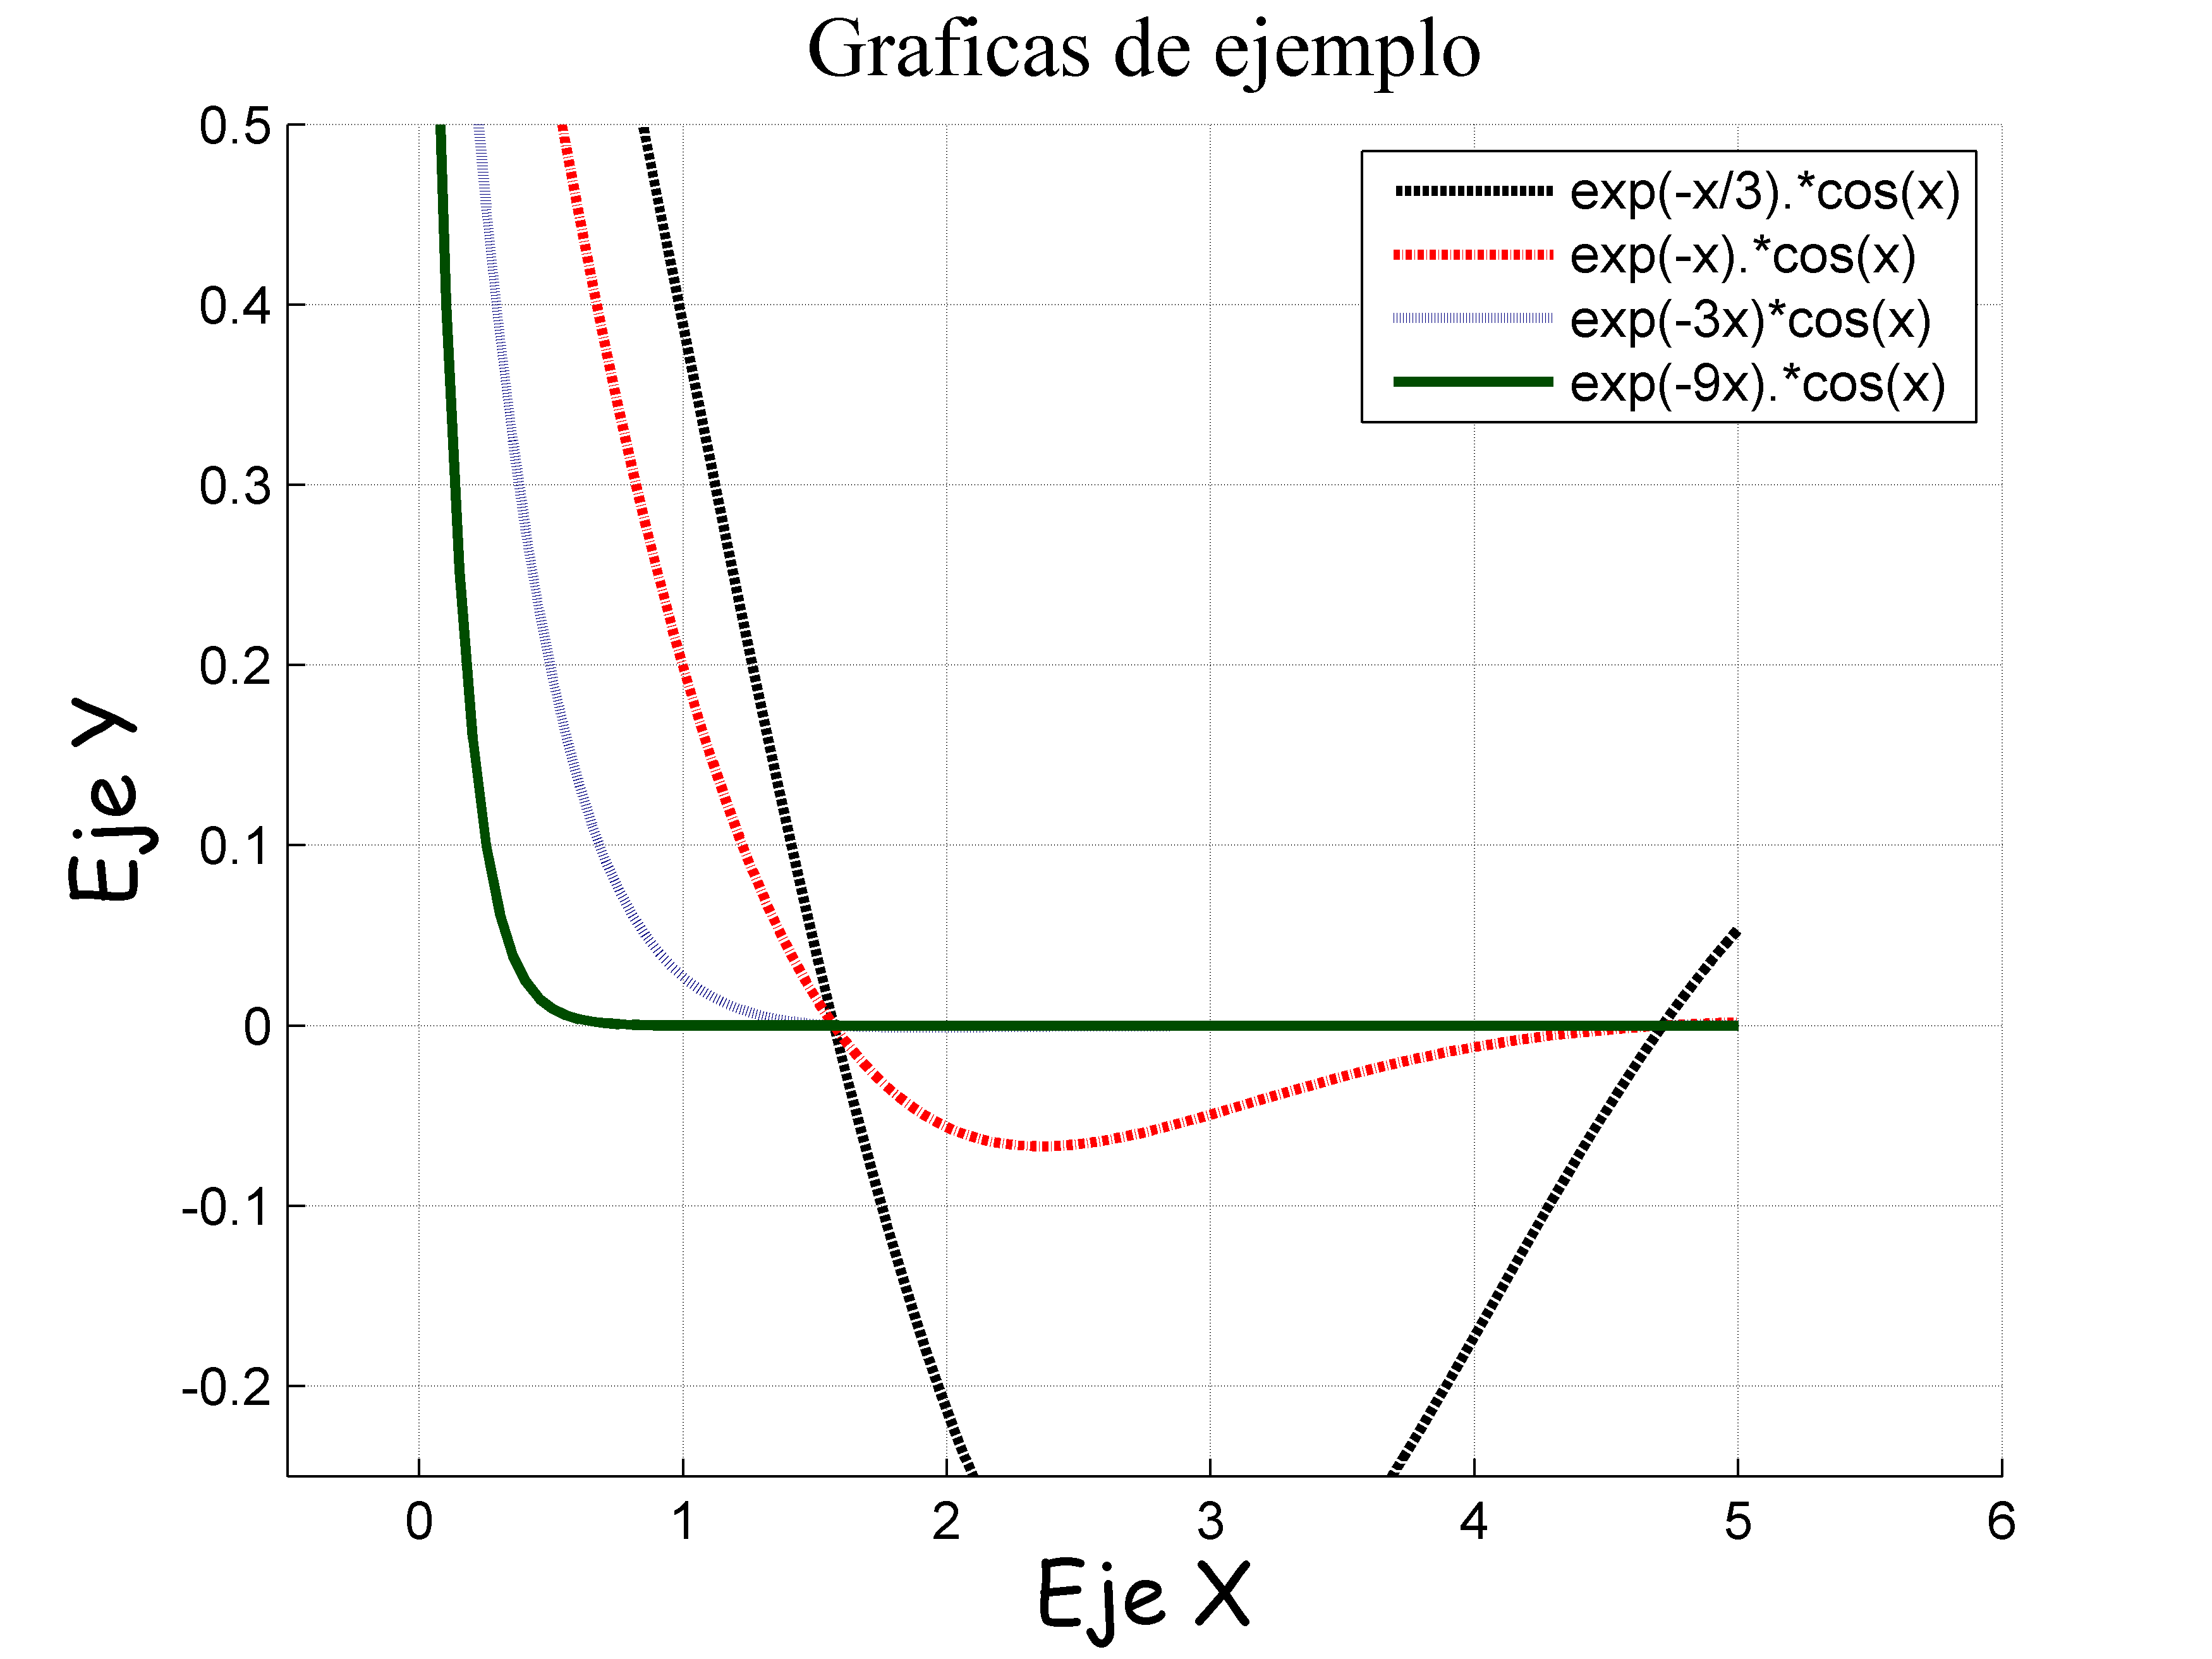
\includegraphics[width=300pt]{./Imagenes/plotas.png}
\end{center}





\section{Otros tipos de salidas gráficas}

Además del comando \textbf{plot}, hay otros comandos que permiten realizar gráficos bi-dimensionales, y que tienen un manejo similar al de este comando. Estos comandos son:

\begin{itemize}
\item \textbf{plotyy}: permite mostrar dos gráficos en la misma ventana con dos ejes Y a la izquierda y a la derecha.
\item \textbf{polar}: curvas en polares
\item \textbf{semilogx, semilogy}: similar a plot, pero usando una escala logarítmica en los ejes X e Y.
\item \textbf{loglog}: escala logarítmica en ambos ejes.
\item \textbf{stem}: dibuja uniéndolos con una linea vertical al eje X.
\item \textbf{stairs}: traza una gráfica en forma de escalera.
\item \textbf{bar, barh, bar3}: despliega gráficas en forma de barras. Útil para representar datos estadísticos.
\item \textbf{area}: muestra los datos en una gráfica d forma acumulada. El color se controla con el comando colormap. 
\item \textbf{line}: un puntos mediante líneas. Instrucción de bajo nivel que da origen a plot.
\item \textbf{fill}: dibuja polígonos cerrados y colora su interior.
\item \textbf{patch}: construye polígonos o caras en 3 dimensiones y asigna un color a la cara definida.
\end{itemize}

\section{Gráficos de funciones}

\textbf{MATLAB} tiene una serie de comandos asociados al Toolbox de calculo simbólico, los cuales nos permiten obtener la gráfica  d las funciones más conocidas. En esa sección podremos observar como quedan representadas las funciones más comunes.

\subsubsection{Función lineal}

\begin{enumerate}

\item \textbf{Ejemplo 1}: función $y = x + 2$
\begin{lstlisting}[language=Matlab]
>> x = [1:1:10]

x =

     1     2     3     4     5     6     7     8     9    10

>> y = x+2;
>> plot(y)
\end{lstlisting}
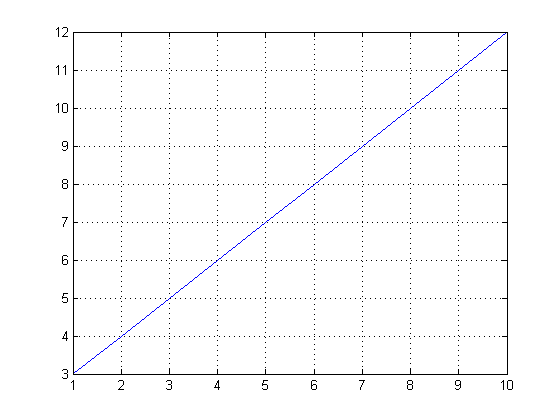
\includegraphics[width=300pt]{./Imagenes/ejem1.png}

\item \textbf{Ejemplo 2}: función $y = -x + 2$
\begin{lstlisting}[language=Matlab]
>> y = -x+2;
>> plot(y)
>> grid
\end{lstlisting}
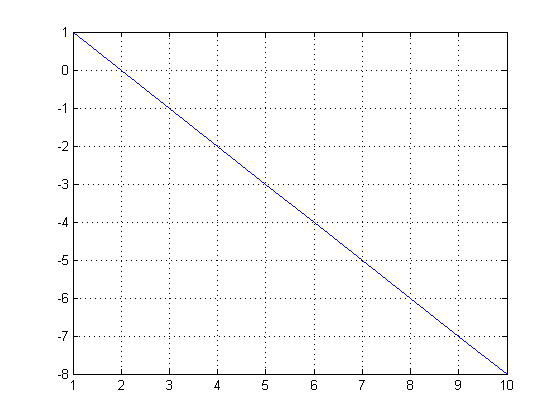
\includegraphics[width=300pt]{./Imagenes/ejem2.png}
\end{enumerate}

\subsubsection{Función raíz cuadrada}

\begin{enumerate}
\item \textbf{Ejemplo 1}: función $y = \sqrt{t}$
\begin{lstlisting}[language=Matlab]
>> t = 0:.05:4*pi;
>> y = sqrt(t);
>> plot(t,y)
>> grid
\end{lstlisting}
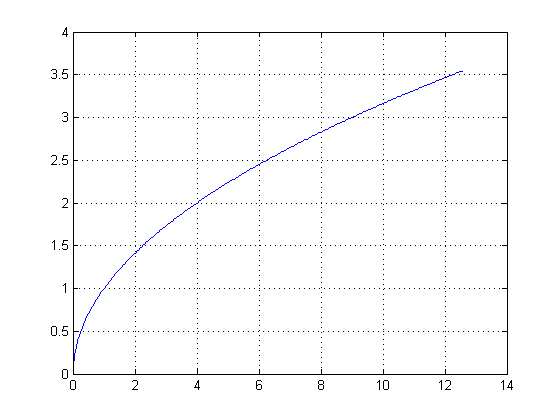
\includegraphics[width=300pt]{./Imagenes/ejem13.png}
\end{enumerate}


\subsubsection{Función exponencial}

\begin{enumerate}

\item \textbf{Ejemplo 1}: función $y = 2^{t}$
\begin{lstlisting}[language=Matlab]
>> t = 0:.05:4*pi;
>> y = 2.^(t);
>> plot(t,y)
>> grid
\end{lstlisting}
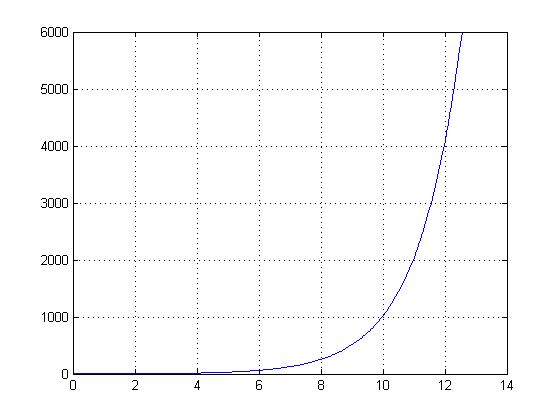
\includegraphics[width=300pt]{./Imagenes/ejem14.png}
\end{enumerate}



\section{Graficar observaciones y predicciones}

Es muy frecuente en ingeniería comparar las observaciones medidas (por ejemplo la temperatura 
ambiente) con los cálculos realizados mediante un modelo matemático (sea éste meramente una 
función algebraica ajustada previamente a los datos, o un modelo teórico que interprete la física del sistema). El siguiente programa ilustra un ejercicio, donde se comparan datos de un día lluvioso, con un polinomio de grado 5 ajustado a ellos. Incidentalmente se muestran las útiles funciones pre-programadas de \textbf{MATLAB}, \textbf{polyfit} que devuelve el vector de coeficientes del polinomio ajustado según el método de los cuadrados mínimos y \textbf{polyval} que calcula los valores del polinomio dado el vector de coeficientes y el vector de la variable 
independiente, t.

\begin{lstlisting}[language=Matlab]
>> clear 
>> t = 0:1:23; 
>> T = [12 11.5 10.9 9.8 9.4 8.7 8.5 8.9 10.1 11.3 12.1 13 14 14.5 14.8 15.1 15.4 15.2... 
        15.1 14.7 14.2 13.9 13.6 12.8 ]; 
>> p = polyfit (t, T,5) 
>  Tp = polyval(p,t) 
>> plot (t,T, 'o', t, Tp, 'Linewidth', 1); 
>> Title ('DIA LLUVIOSO', 'Fontsize', 25) 
>> xlabel ('Hora', 'Fontsize', 20) 
>> ylabel ('Temperatura', 'Fontsize', 20) 
>> legend ('Datos del SMN', 'Polynomio grado 5') 
\end{lstlisting}
\begin{center}
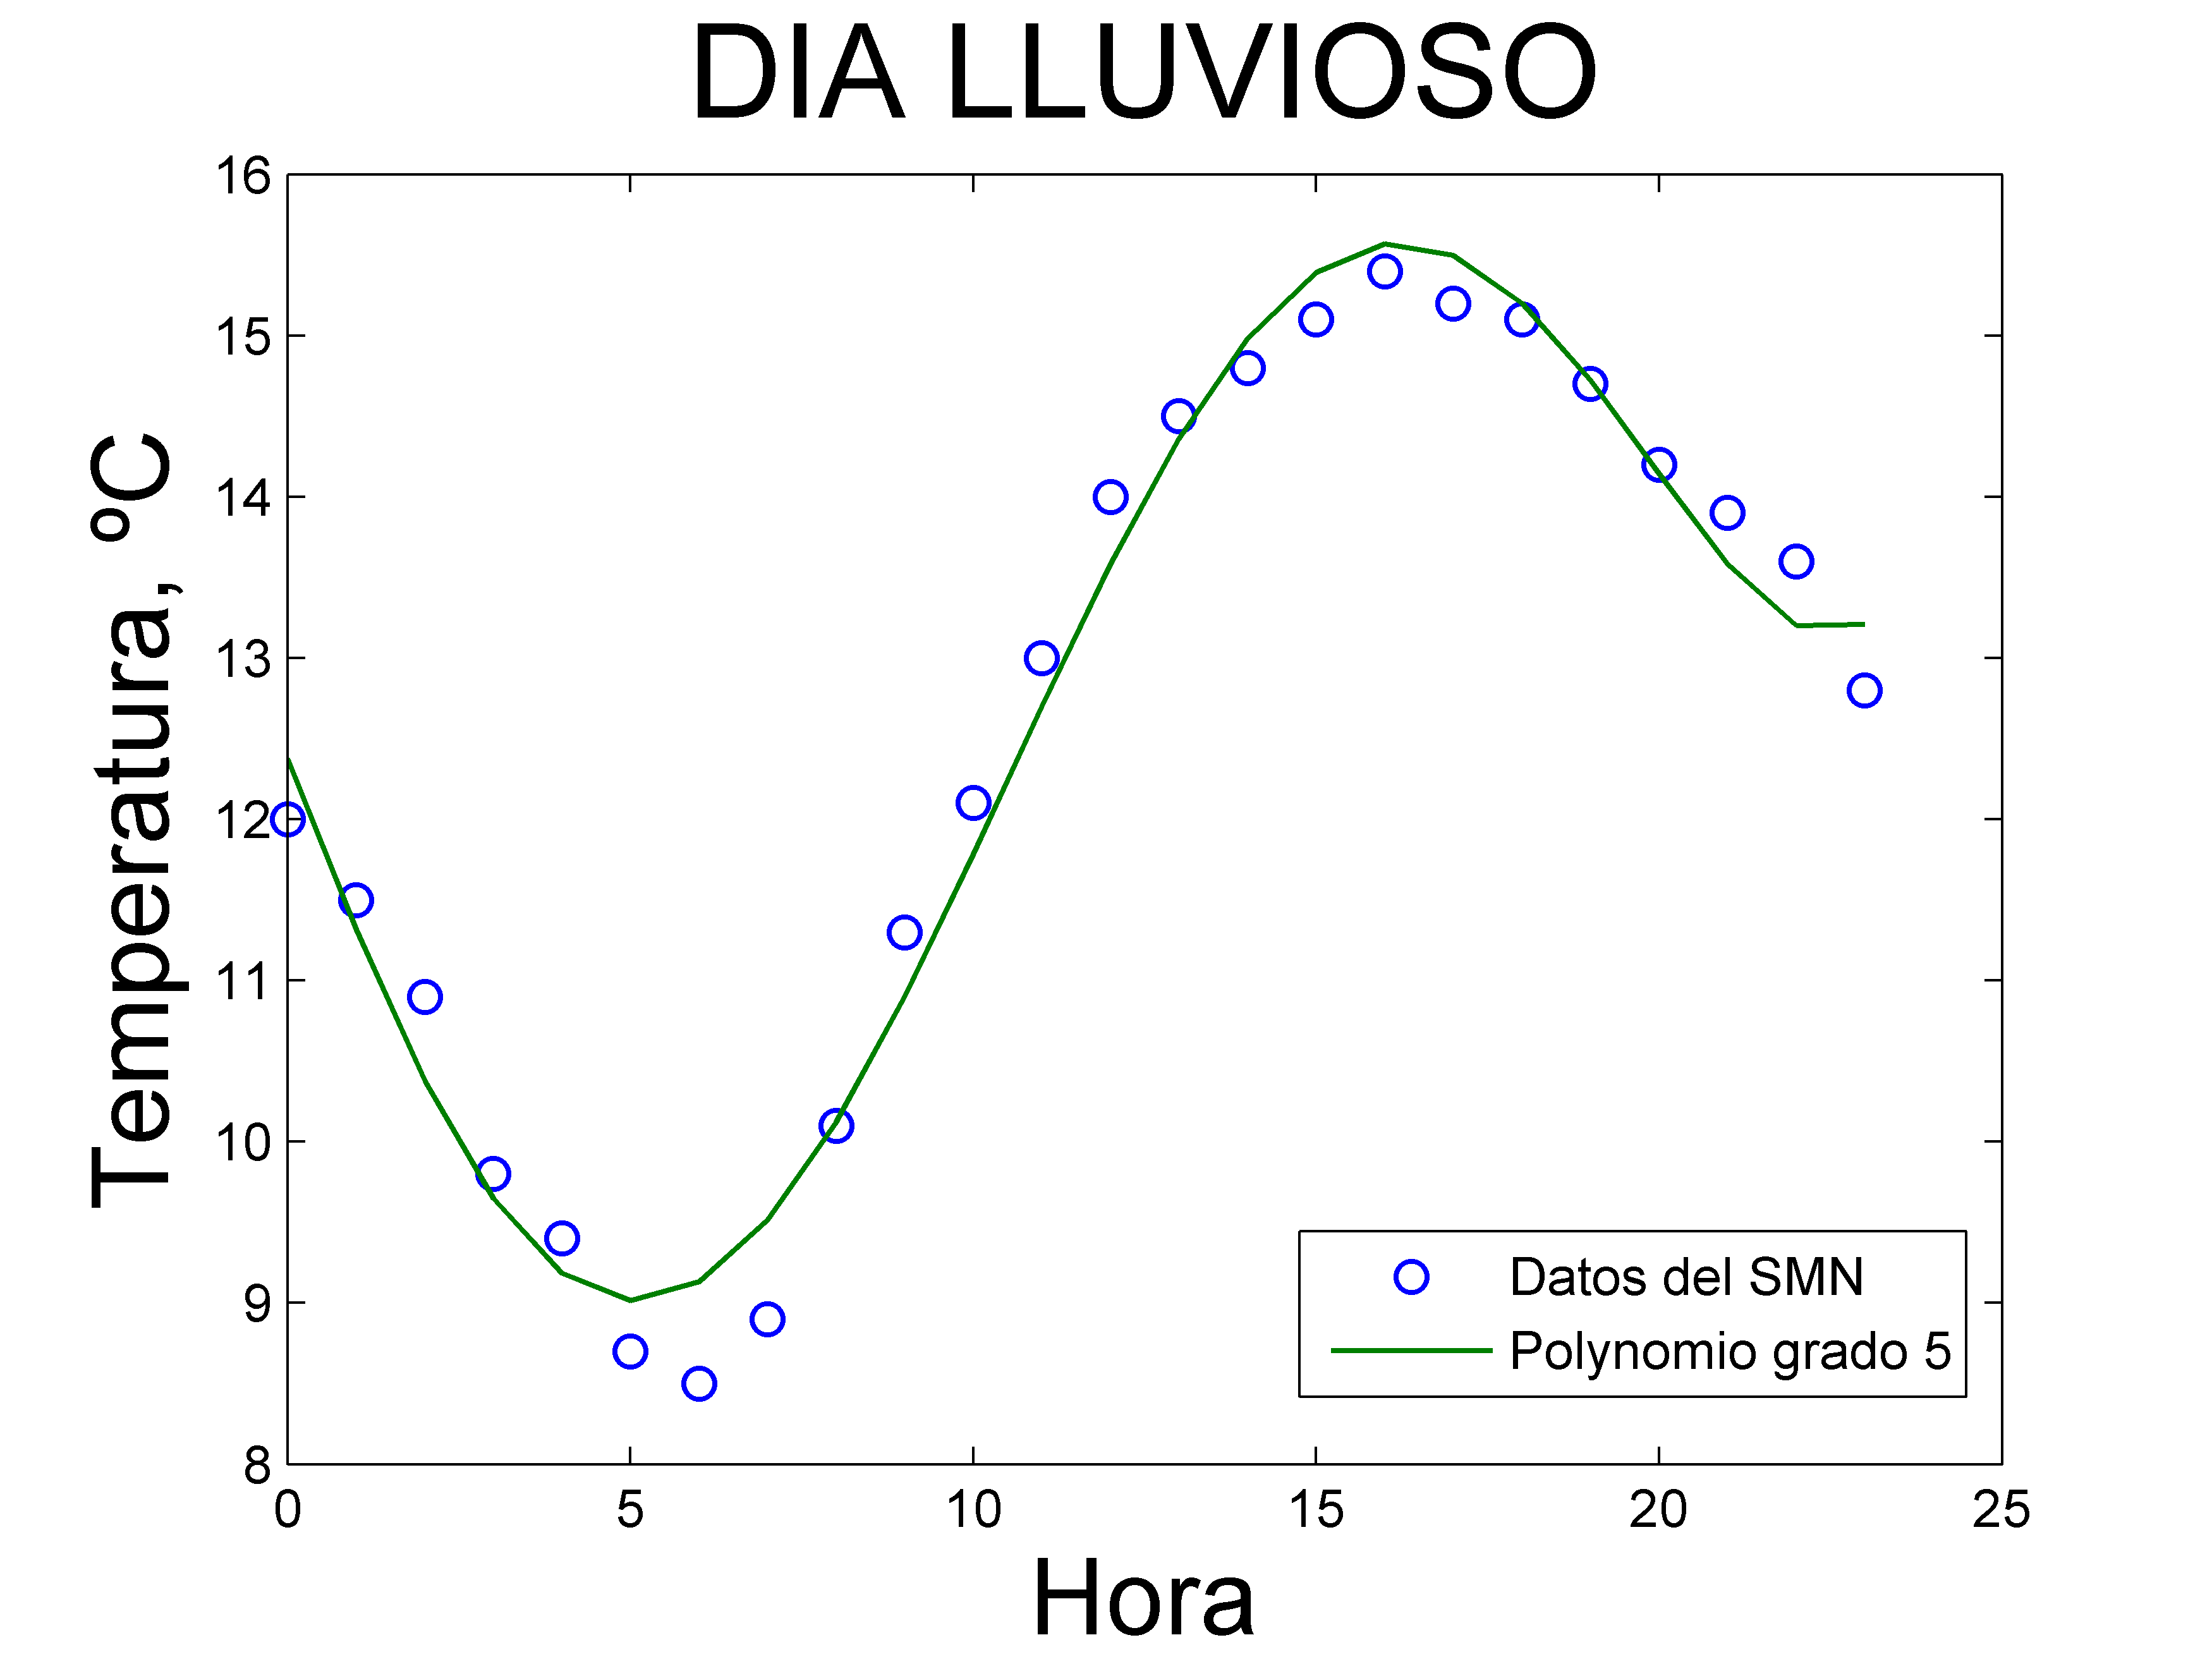
\includegraphics[width=300pt]{./Imagenes/polyfit.png}
\end{center}

\section{Otros comandos}

\begin{enumerate}

\item \textbf{linspace} y \textbf{fplot}: sea la función $f(x)=e^{-x}$, si $-2 \leq x \leq 3$. La gráfica en \textbf{MATLAB} de esta función se obtiene en tres pasos. Primero, mediante el comando \textbf{linspace} se divide el intervalo [-2,3] en 3000 partes. Luego definimos la función y finalmente utilizamos el comando \textbf{plot}.

\begin{lstlisting}[language=Matlab]
>> x=linspace(-2,3,3000);
>> y=exp(-x);
>> plot(x,y);
>> grid on;
\end{lstlisting}
\begin{center}
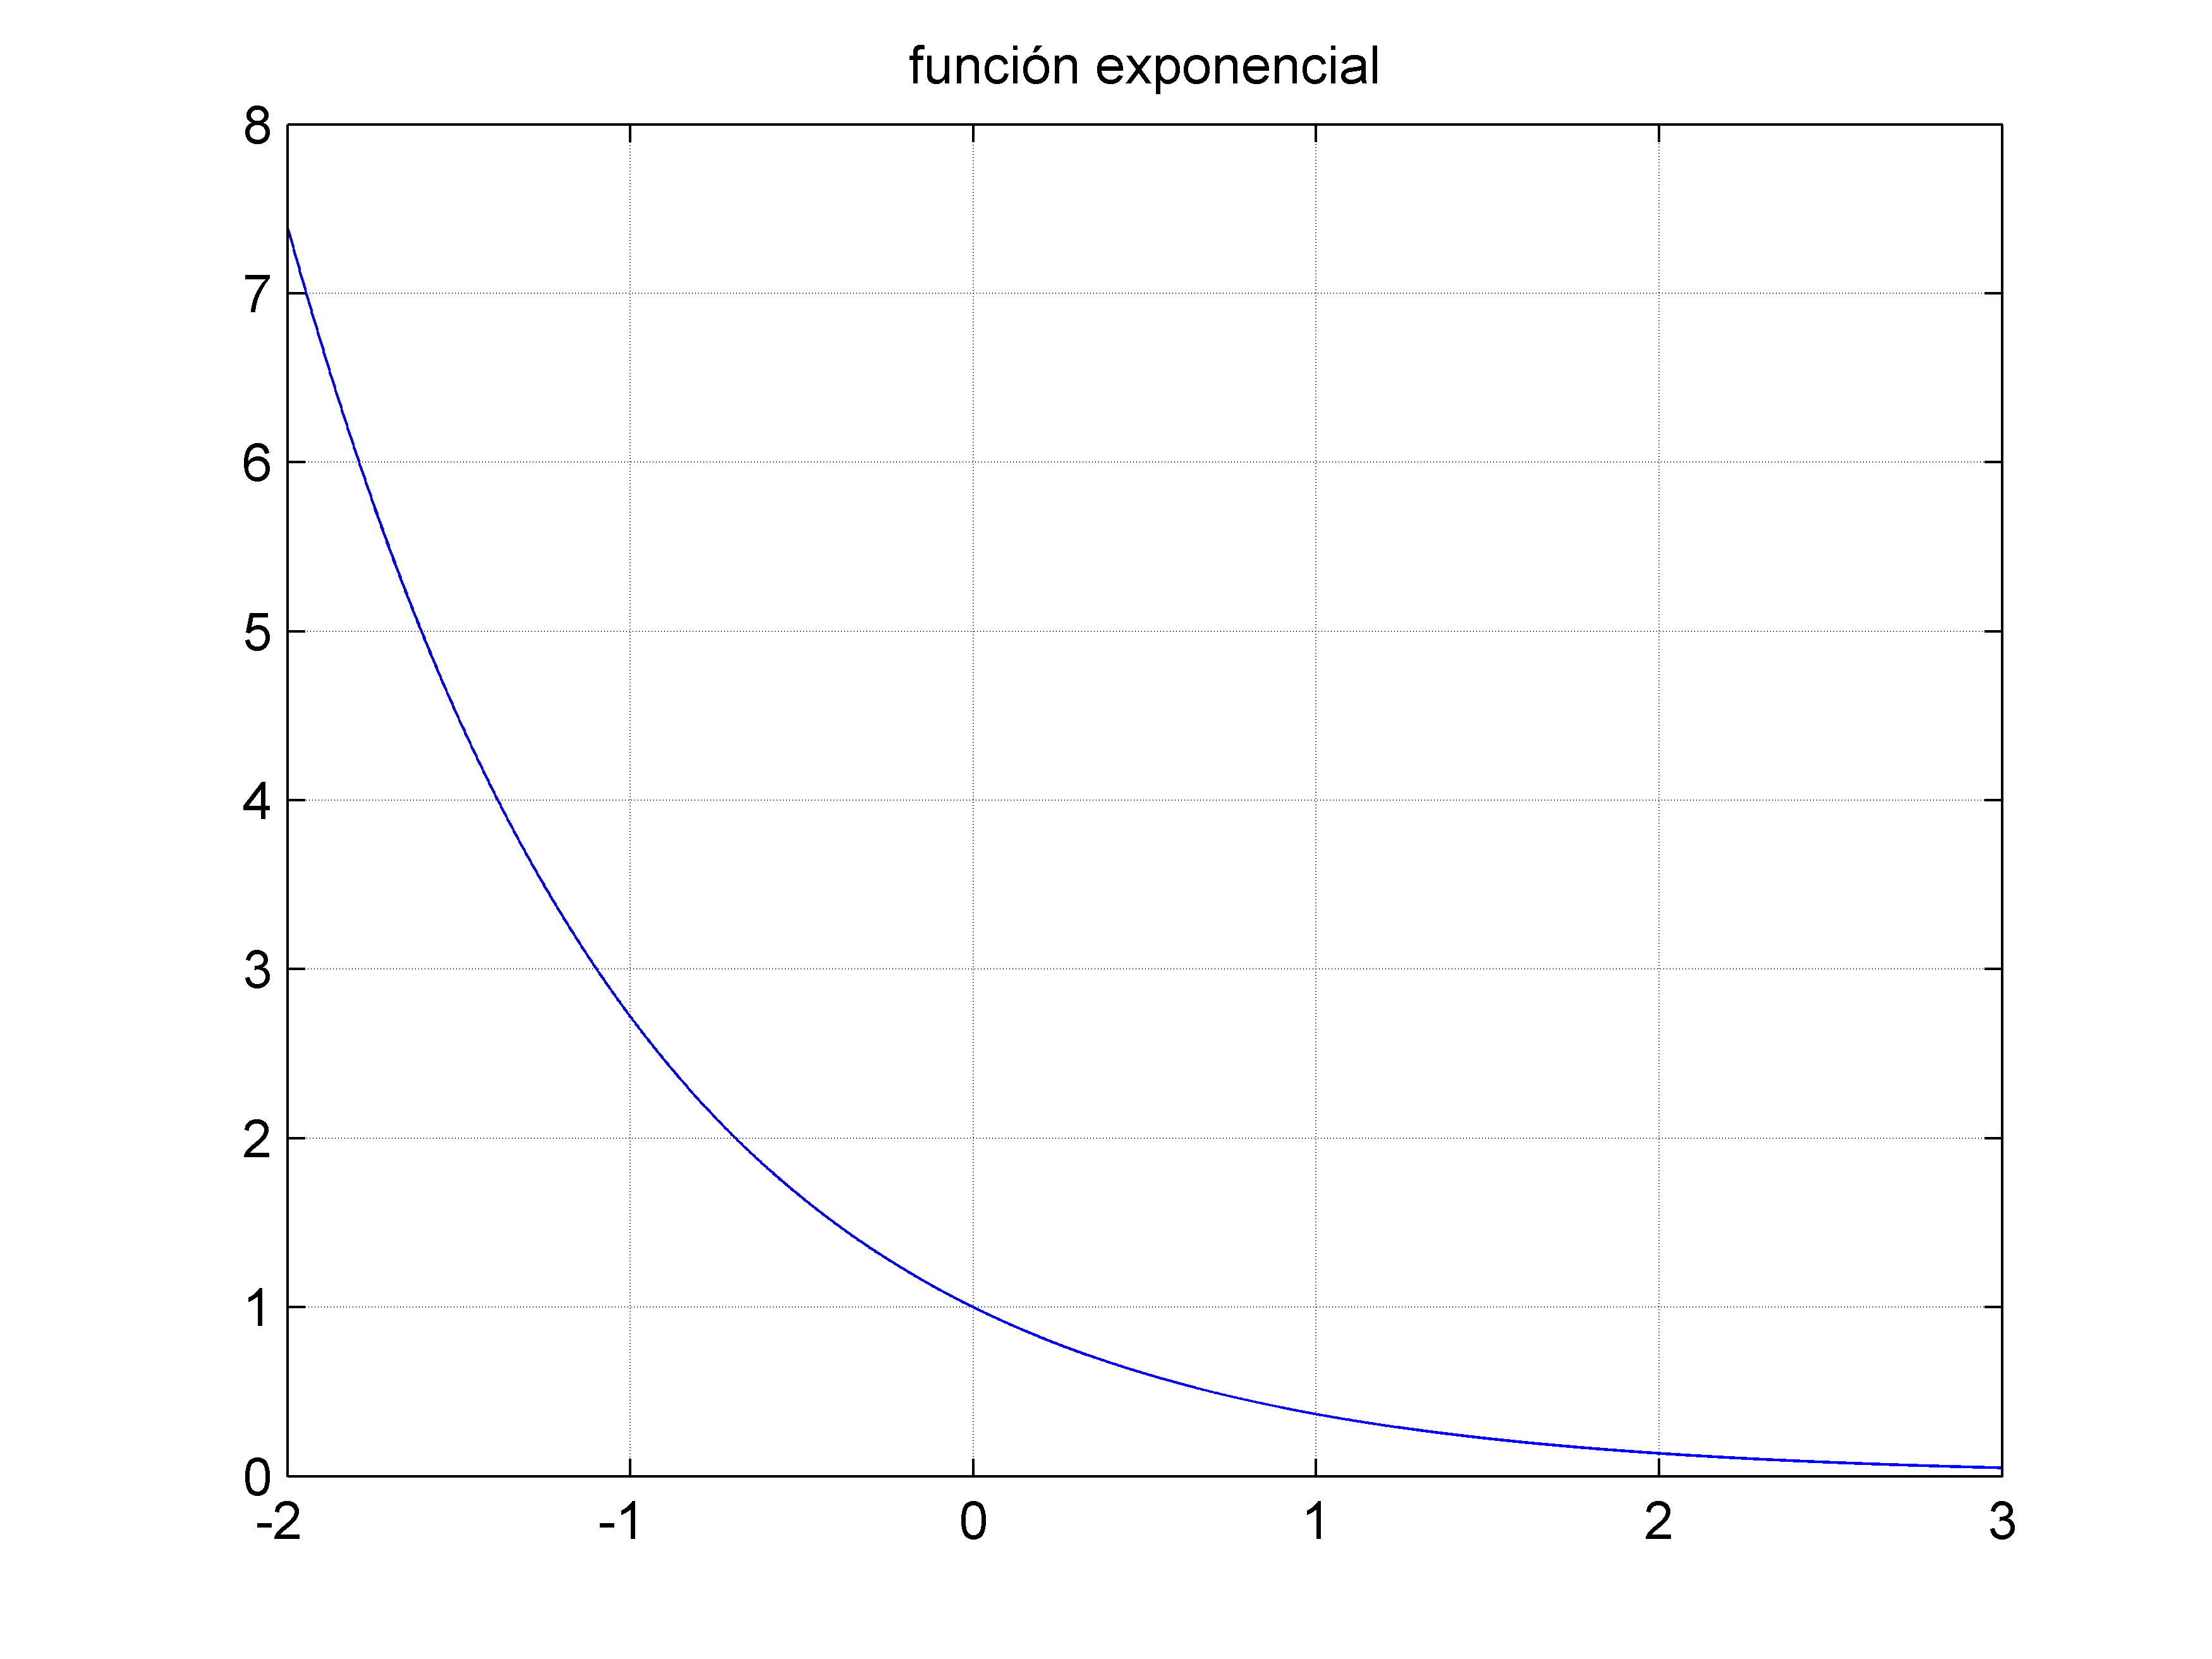
\includegraphics[width=300pt]{./Imagenes/linspace.png}
\end{center} 

Existe otra forma de representar $f$ en un solo paso:
\begin{lstlisting}[language=Matlab]
>> fplot('exp(-x)',[-2,3])
\end{lstlisting}



\item \textbf{Catenaria}: La función que describe esta curva es  $f(x)=cosh(x)$ en el intervalo [-5,5]. Su gráfica se obtiene directamente con la siguiente secuencia de comandos. Primero dividimos el intervalo [-5:5] en pequeños intervalos de 0.1 de longitud. Luego evaluamos $f$ en cada punto \textbf{x} de la división. Finalmente generamos el gráfico.

\begin{lstlisting}[language=Matlab]
>> x=-5:0.1:5;
>> y=cosh(x); 
>> plot(x,y)
\end{lstlisting}
\begin{center}
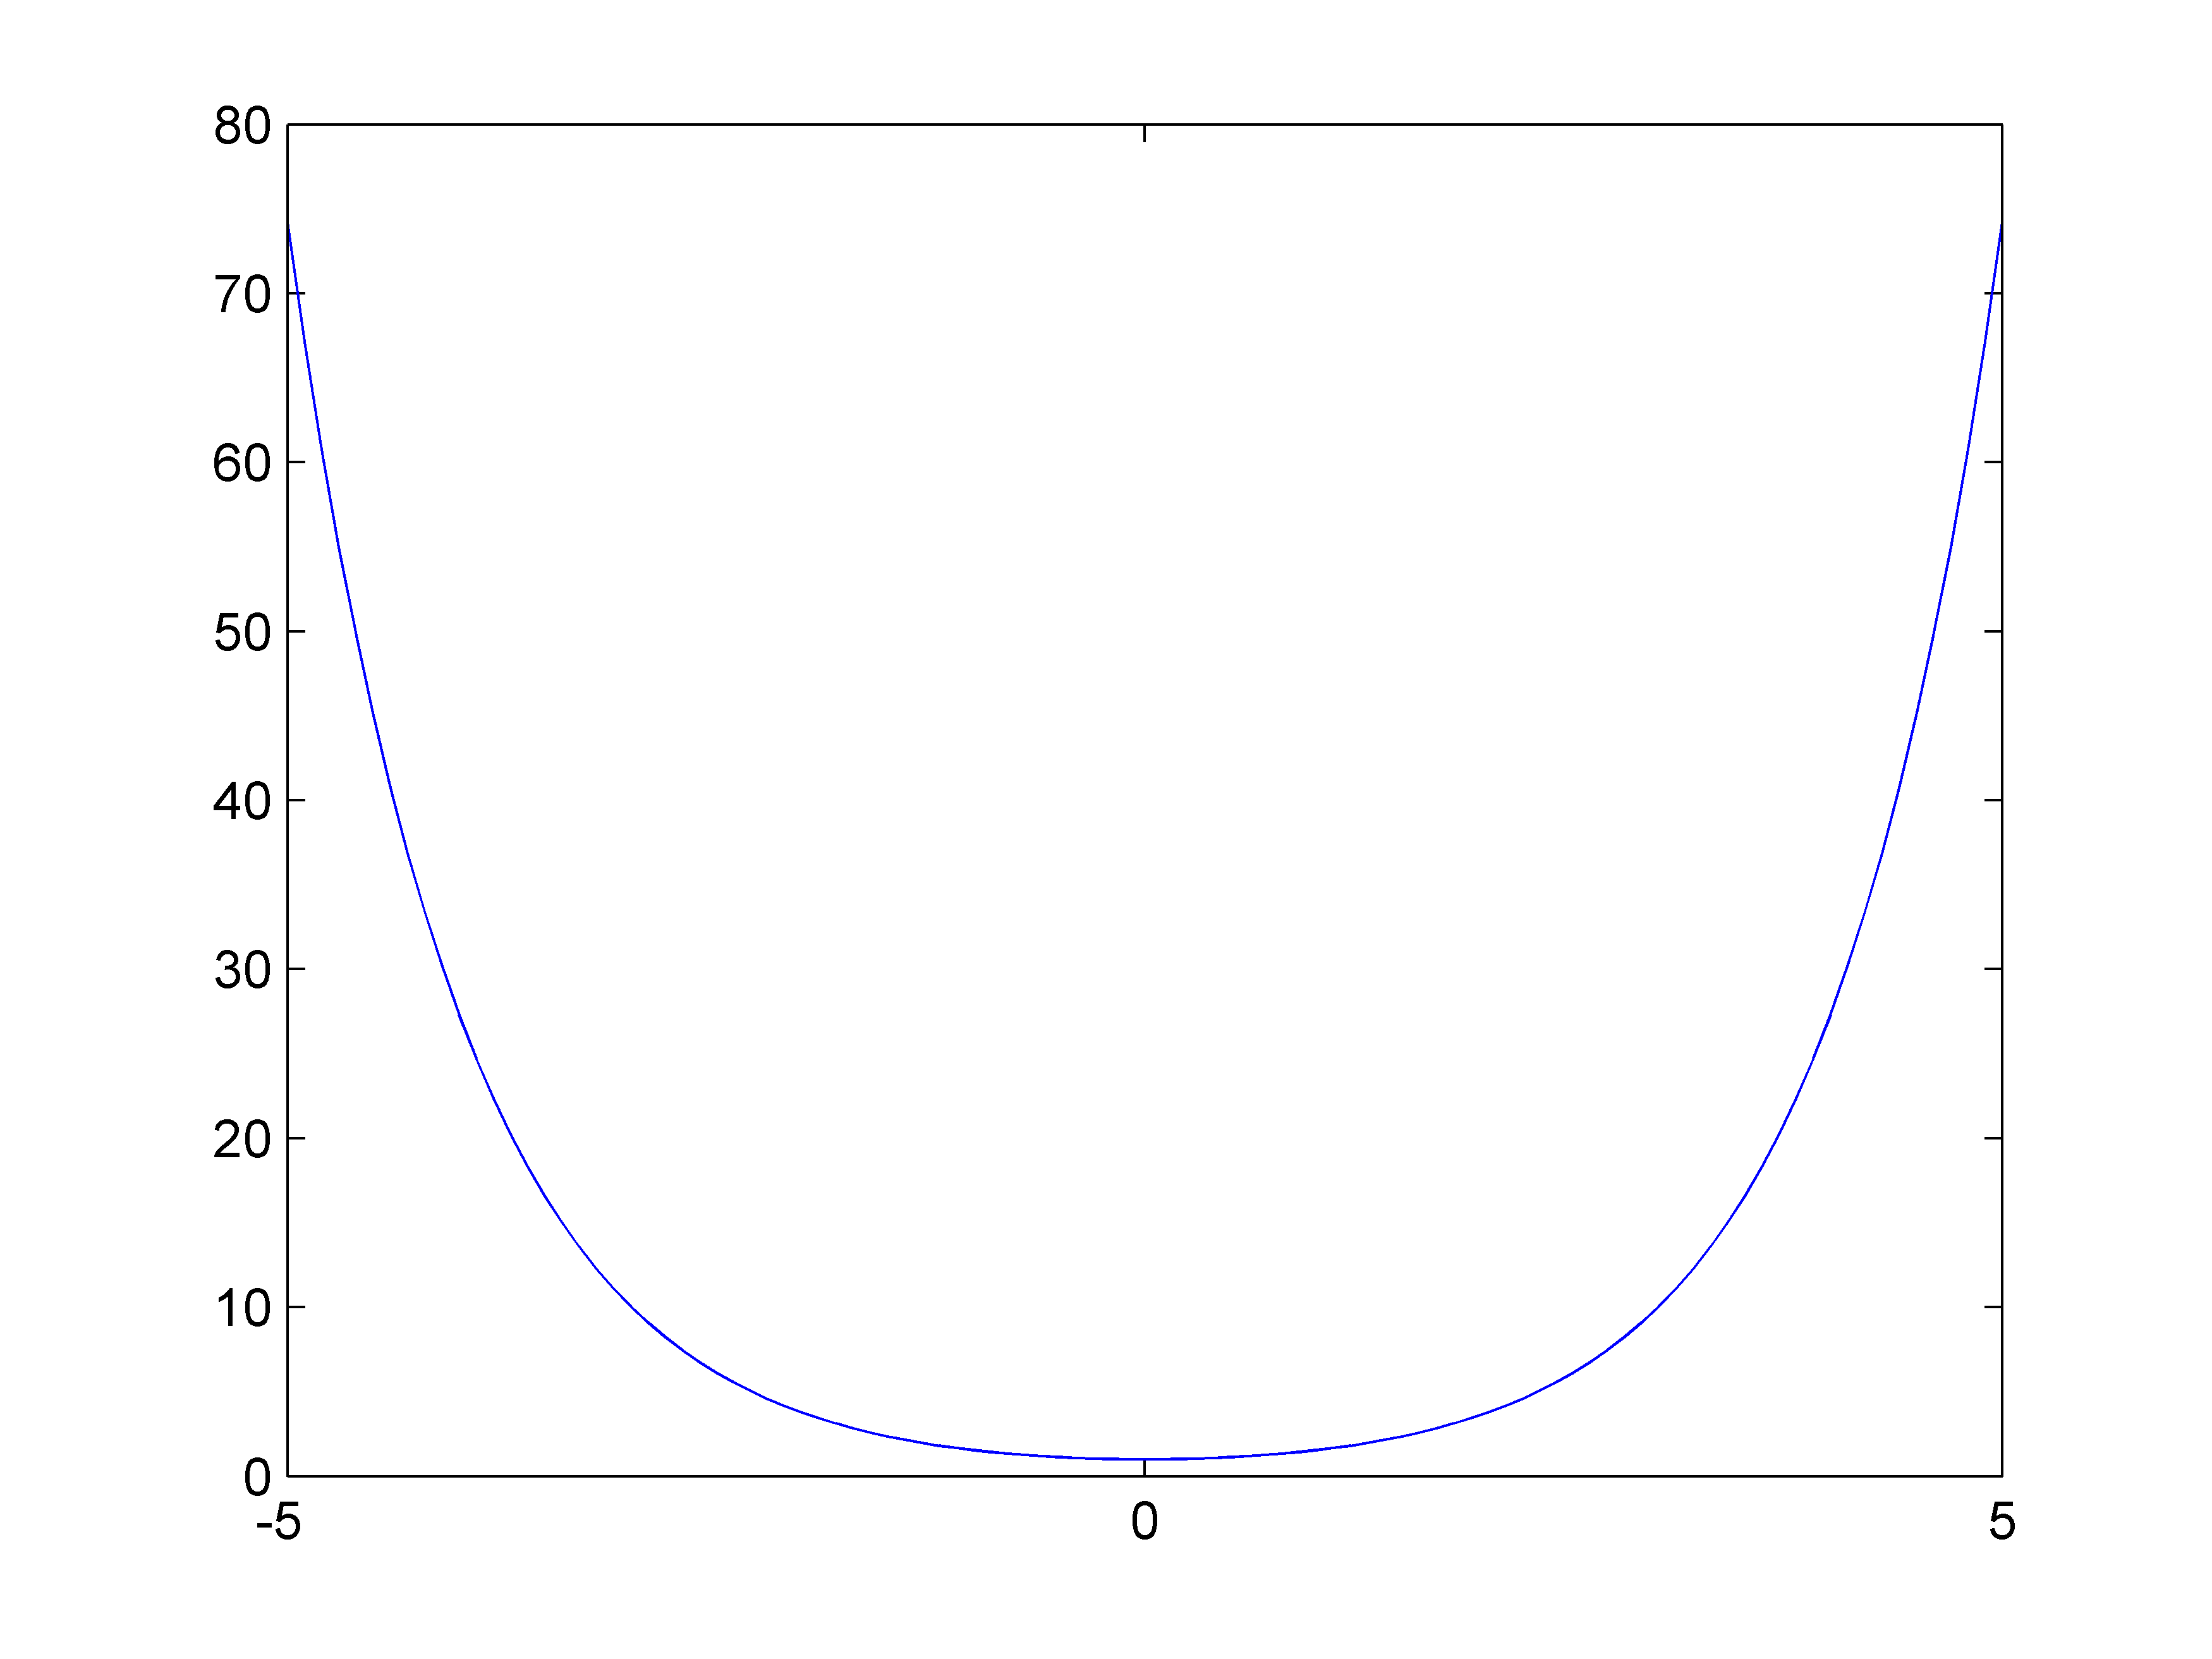
\includegraphics[width=300pt]{./Imagenes/catenaria.png}
\end{center} 


\item Funciones seccionadas usando comandos lógicos. Consideremos la función:

$$
f(n) = \left \{ \begin{matrix} x^{2} & x < 0
\\ 2 & 0 \leqslant x < 1
\\ -x+3 & 1 \leqslant x \end{matrix}\right. 
$$

Para generar el gráfico primero dividimos el intervalo [-2,3] en 3000 partes y luego evaluamos $f$ usando índice lógico:

\begin{lstlisting}[language=Matlab]
>> x=linspace(-2,3,3000);  
>> y=(x.^2).*(x<0)+2.*((0<=x)&(x<1))+(-x+3).*(1<=x); 
>> plot(x,y)
\end{lstlisting}
\begin{center}
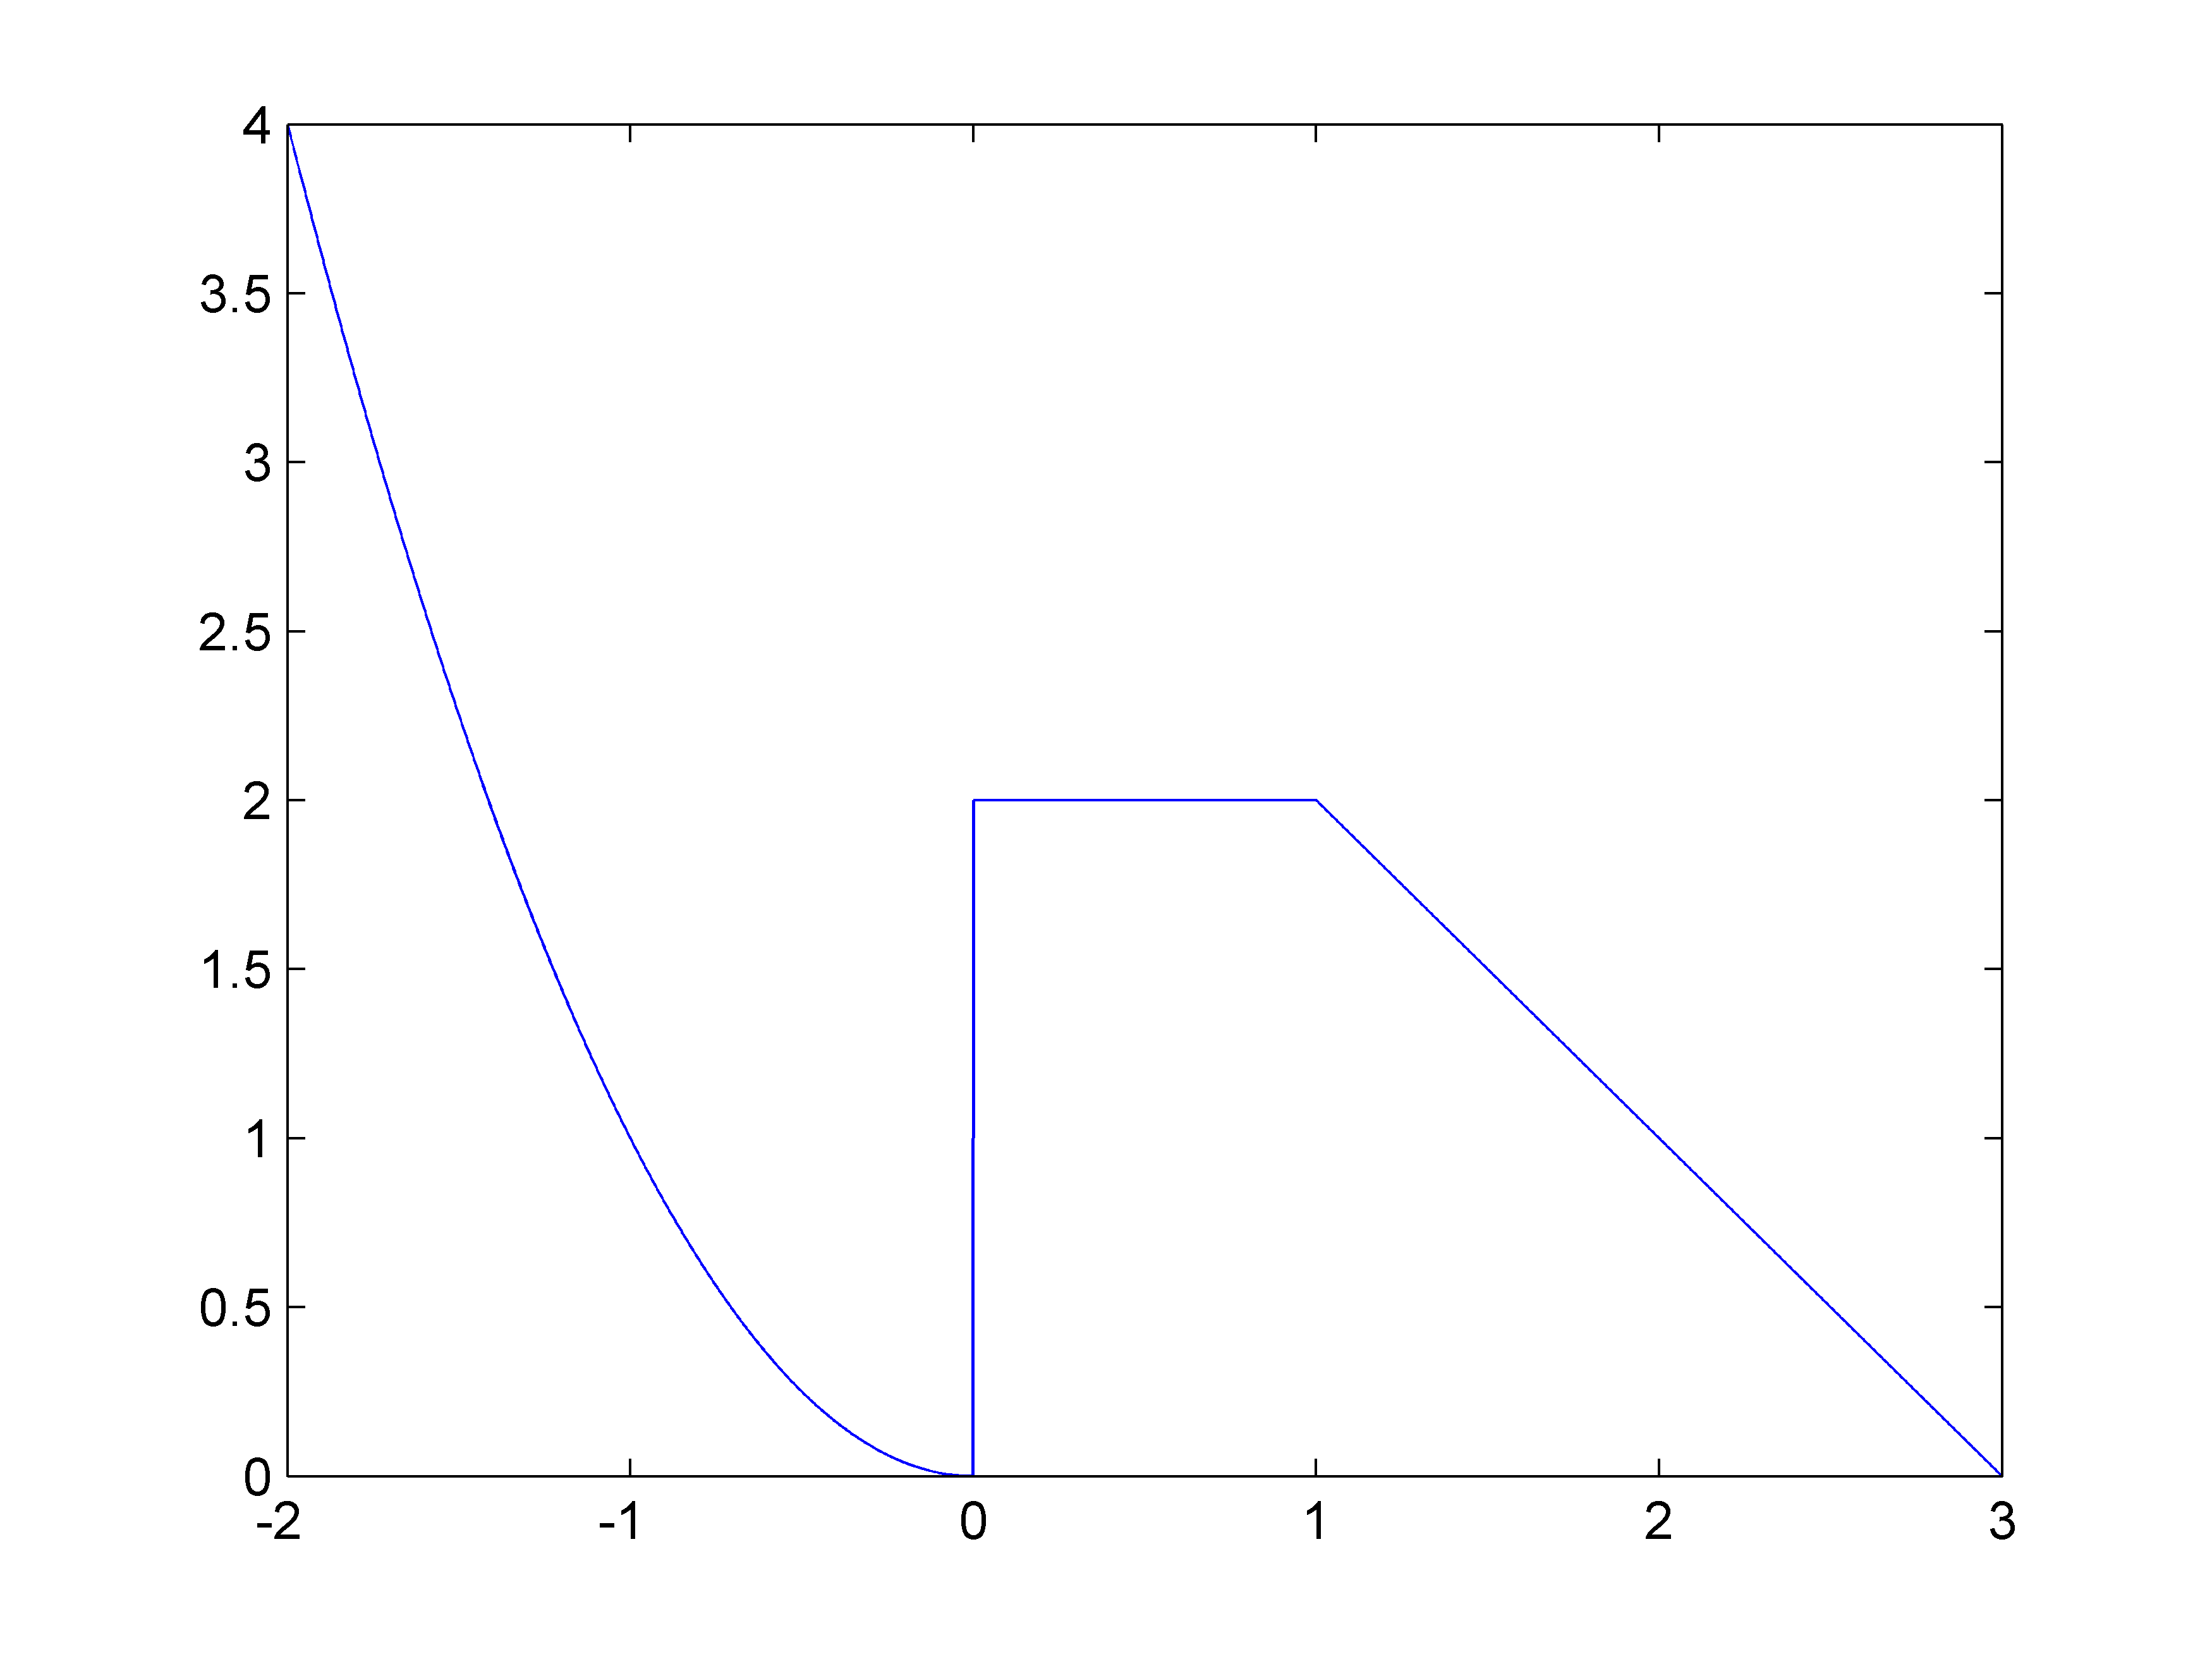
\includegraphics[width=300pt]{./Imagenes/variasf.png}
\end{center} 

\end{enumerate}

\section{Curvas en coordenadas paramétricas}
 
Sea $F(x,y)=0$ con \textbf{x} e \textbf{y} reales, la ecuación cartesiana de una curva C. Si tanto \textbf{x} como \textbf{y} son funciones de una tercera variable \textbf{t}, $t \in I=[a,b]$ , entonces la curva queda representada por

$$
C : \left \{ \begin{matrix} x = x(t)
\\ y = y(t)' \end{matrix}\right. 
$$

denominadas ecuaciones paramétricas de \textbf{C} y \textbf{t} el parámetro. Para cada valor de \textbf{t}, las ecuaciones paramétricas determinan valores correspondientes de \textbf{x} y de 
\textbf{y}, siendo \textbf{(x;y)} un punto de la curva.

\begin{enumerate}

\item Sea la curva con ecuaciones paramétricas:
$$
C : \left \{ \begin{matrix} x(t) = 4cos(t) - cos(4t) & t \in [0,2\pi]
\\ y(t) = 4sen(t) - sen(4t) \end{matrix}\right. 
$$
\begin{lstlisting}[language=Matlab]
>> t=0:0.1:2*pi; 
>> x=4*cos(t)-cos(4*t);  
>> y=4*sin(t)-sin(4*t);  
>> plot(x,y)
\end{lstlisting}
\begin{center}
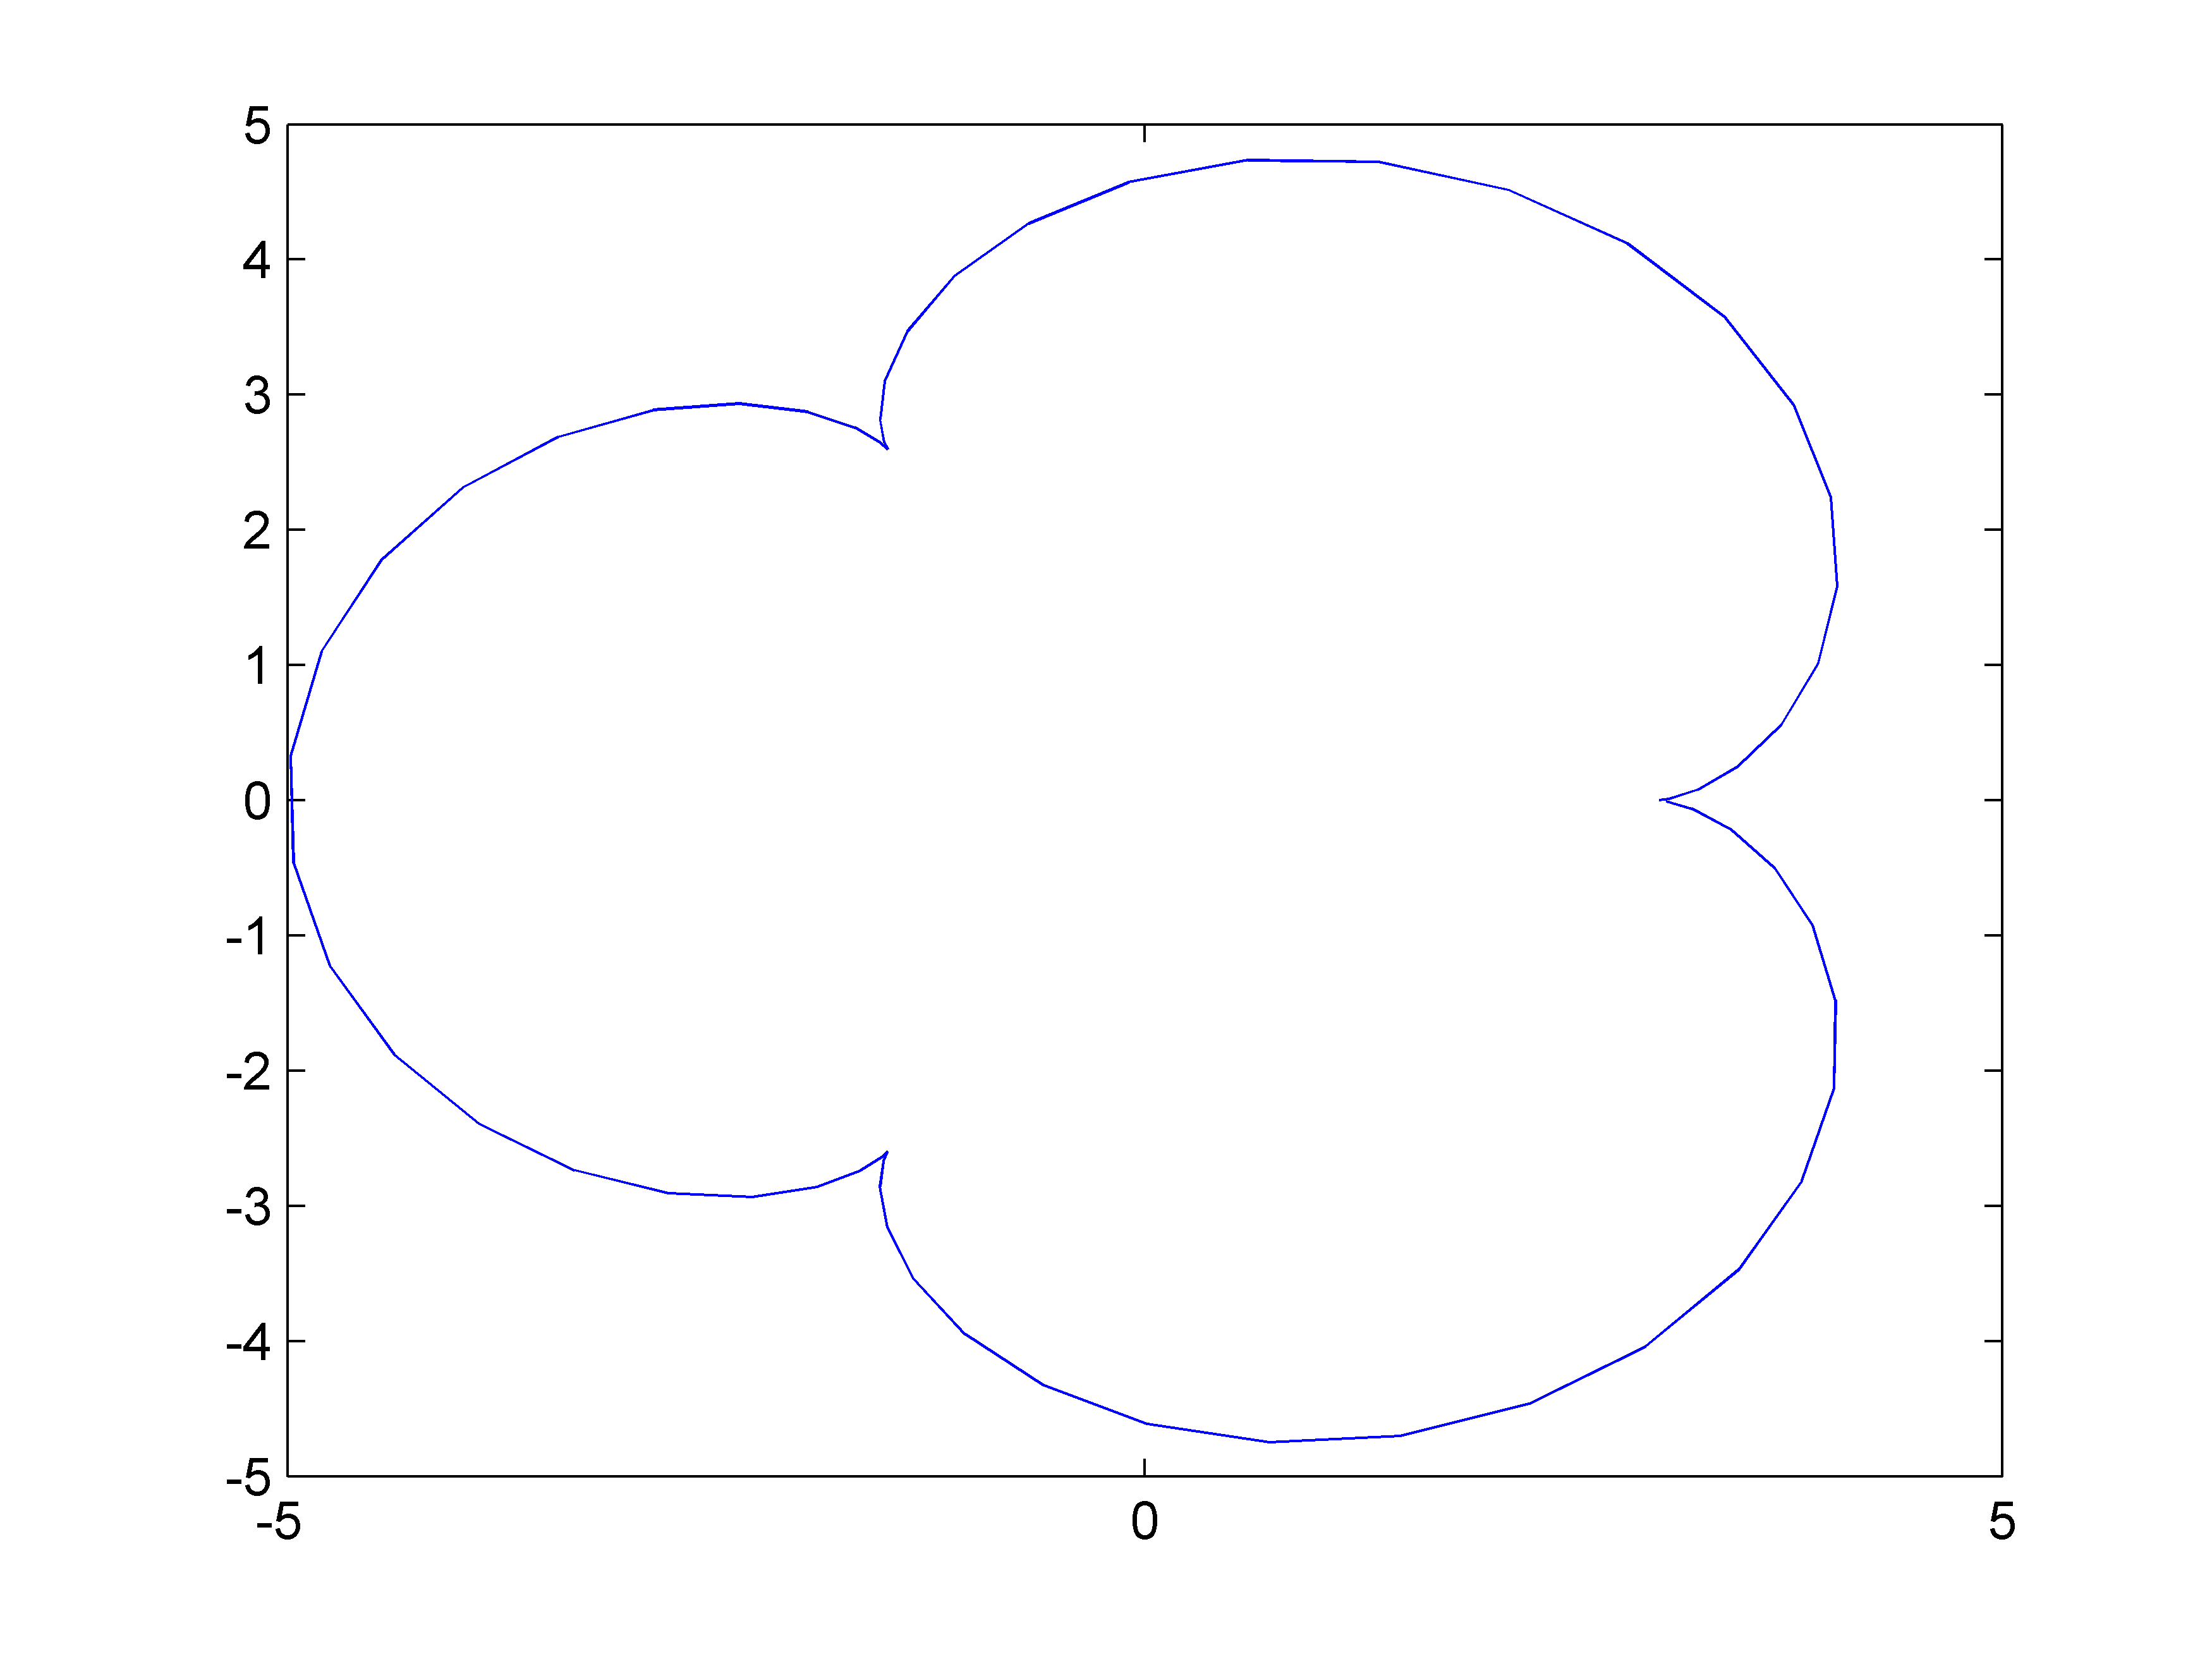
\includegraphics[width=300pt]{./Imagenes/param1.png}
\end{center}

\item Sea C la semicircunferencia unitaria con ecuaciones paramétricas:
$$
C : \left \{ \begin{matrix} x(t) = cos(t) & t \in [0,\pi]
\\ y(t) = sen(t) \end{matrix}\right. 
$$
\begin{lstlisting}[language=Matlab]
>> t=linspace(0,pi,30); 
>> plot(cos(t),sin(t))
\end{lstlisting}
\begin{center}
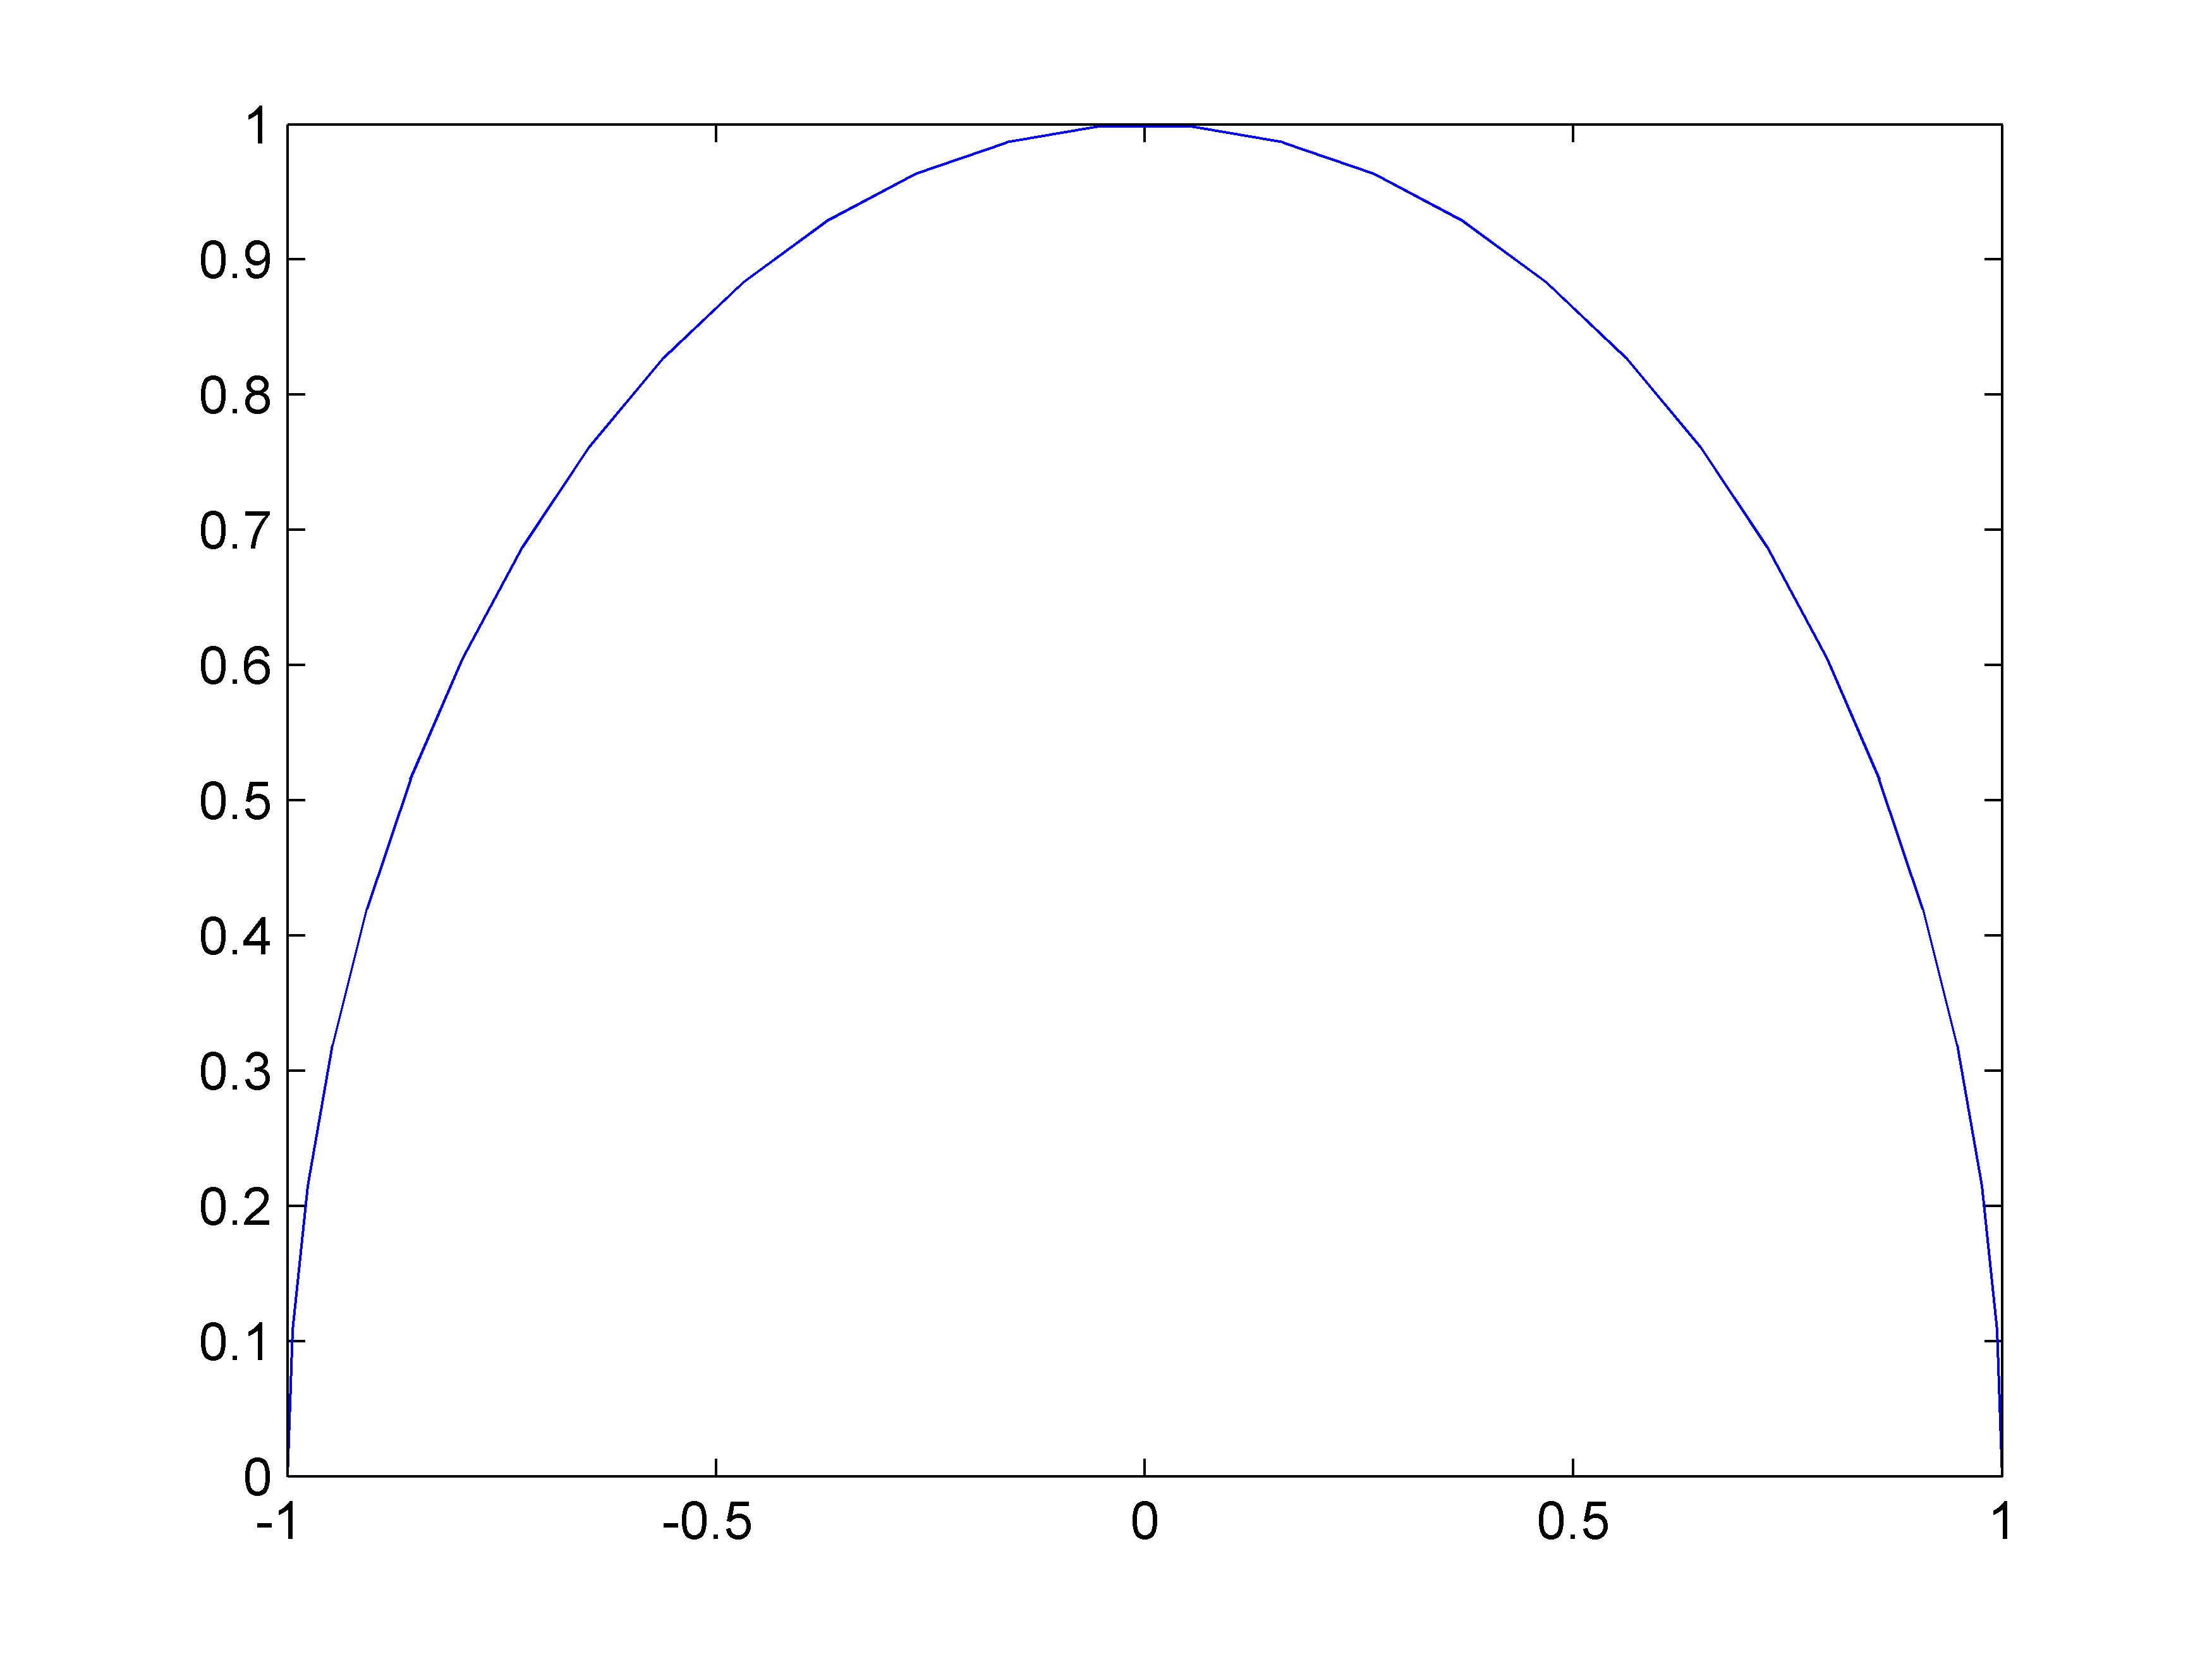
\includegraphics[width=300pt]{./Imagenes/param2.png}
\end{center} 


\item Vectores tangentes a la semicircunferencia anterior en 10 puntos de la curva. A la semicircunferencia anterior le adicionamos los vectores tangentes de la siguiente forma:
\begin{lstlisting}[language=Matlab]
>> t=linspace(0,pi,30); 
>> plot(cos(t),sin(t));
>> hold on  
>> t=linspace(0,pi,10); 
>> quiver(cos(t),sin(t),-sin(t),cos(t)
\end{lstlisting}
\begin{center}
\includegraphics[width=300pt]{./Imagenes/param3.png}
\end{center} 
\end{enumerate}

\section{Curvas en coordenadas polares}

Las coordenadas polares de un punto \textbf{P} las denotaremos por $(r,\theta)$, donde $r$ representa el radio vector y $\theta$ el ángulo polar. Ejemplos:

\begin{enumerate}

\item \textbf{Cardioide}: Ecuación $ r = 1+cos(\theta) donde 0 \leqslant \theta \leqslant 2\pi$. Directamente en la ventana de comandos escribimos:

\begin{lstlisting}[language=Matlab]
>> teta=linspace(0,2*pi,60);
>> r=1+cos(teta);
>> polar(teta,r)
\end{lstlisting}
\begin{center}
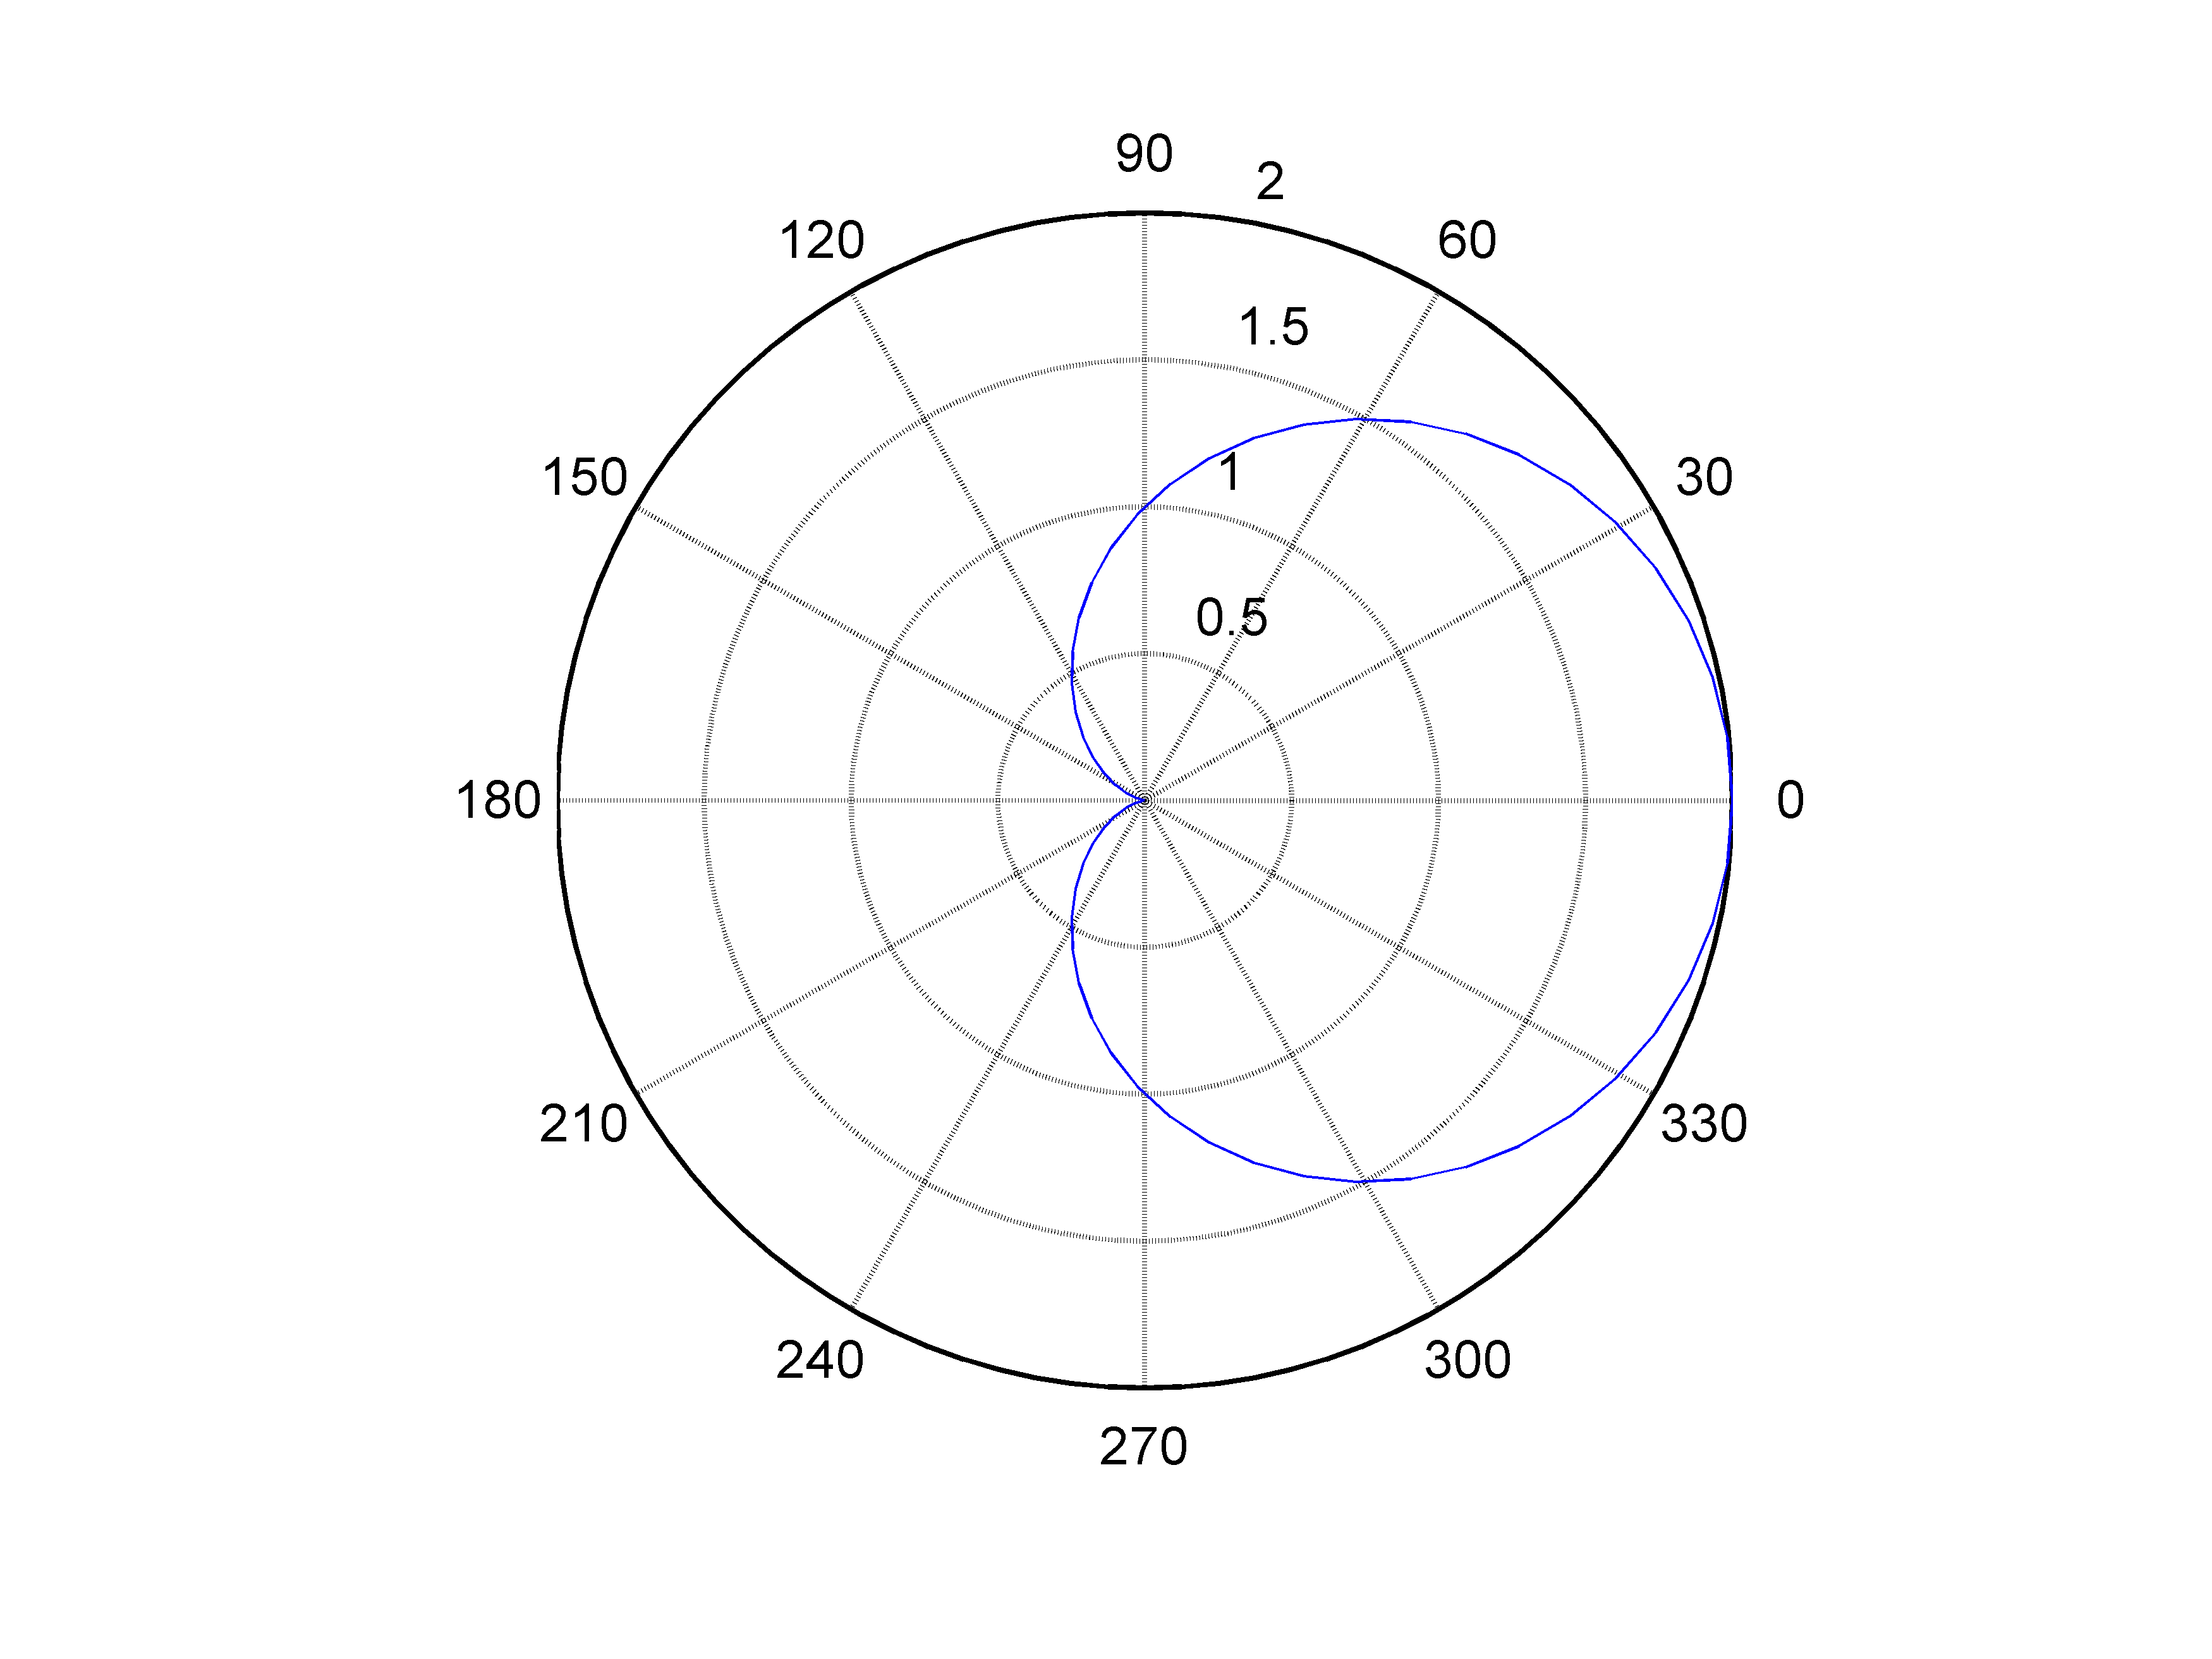
\includegraphics[width=300pt]{./Imagenes/polar1.png}
\end{center} 
 

\item 2. \textbf{Lemniscata de Bernoulli}: de ecuación $r^{2} = 4cos(2\theta), 0 \leqslant \theta \leq 2\pi$. 
La grafica se obtiene mediante los siguientes comandos:

\begin{lstlisting}[language=Matlab]
>> theta=linspace(0,2*pi,300); 
>> r=sqrt(4*cos(2*theta)); 
>> polar(theta,r)
\end{lstlisting}
\begin{center}
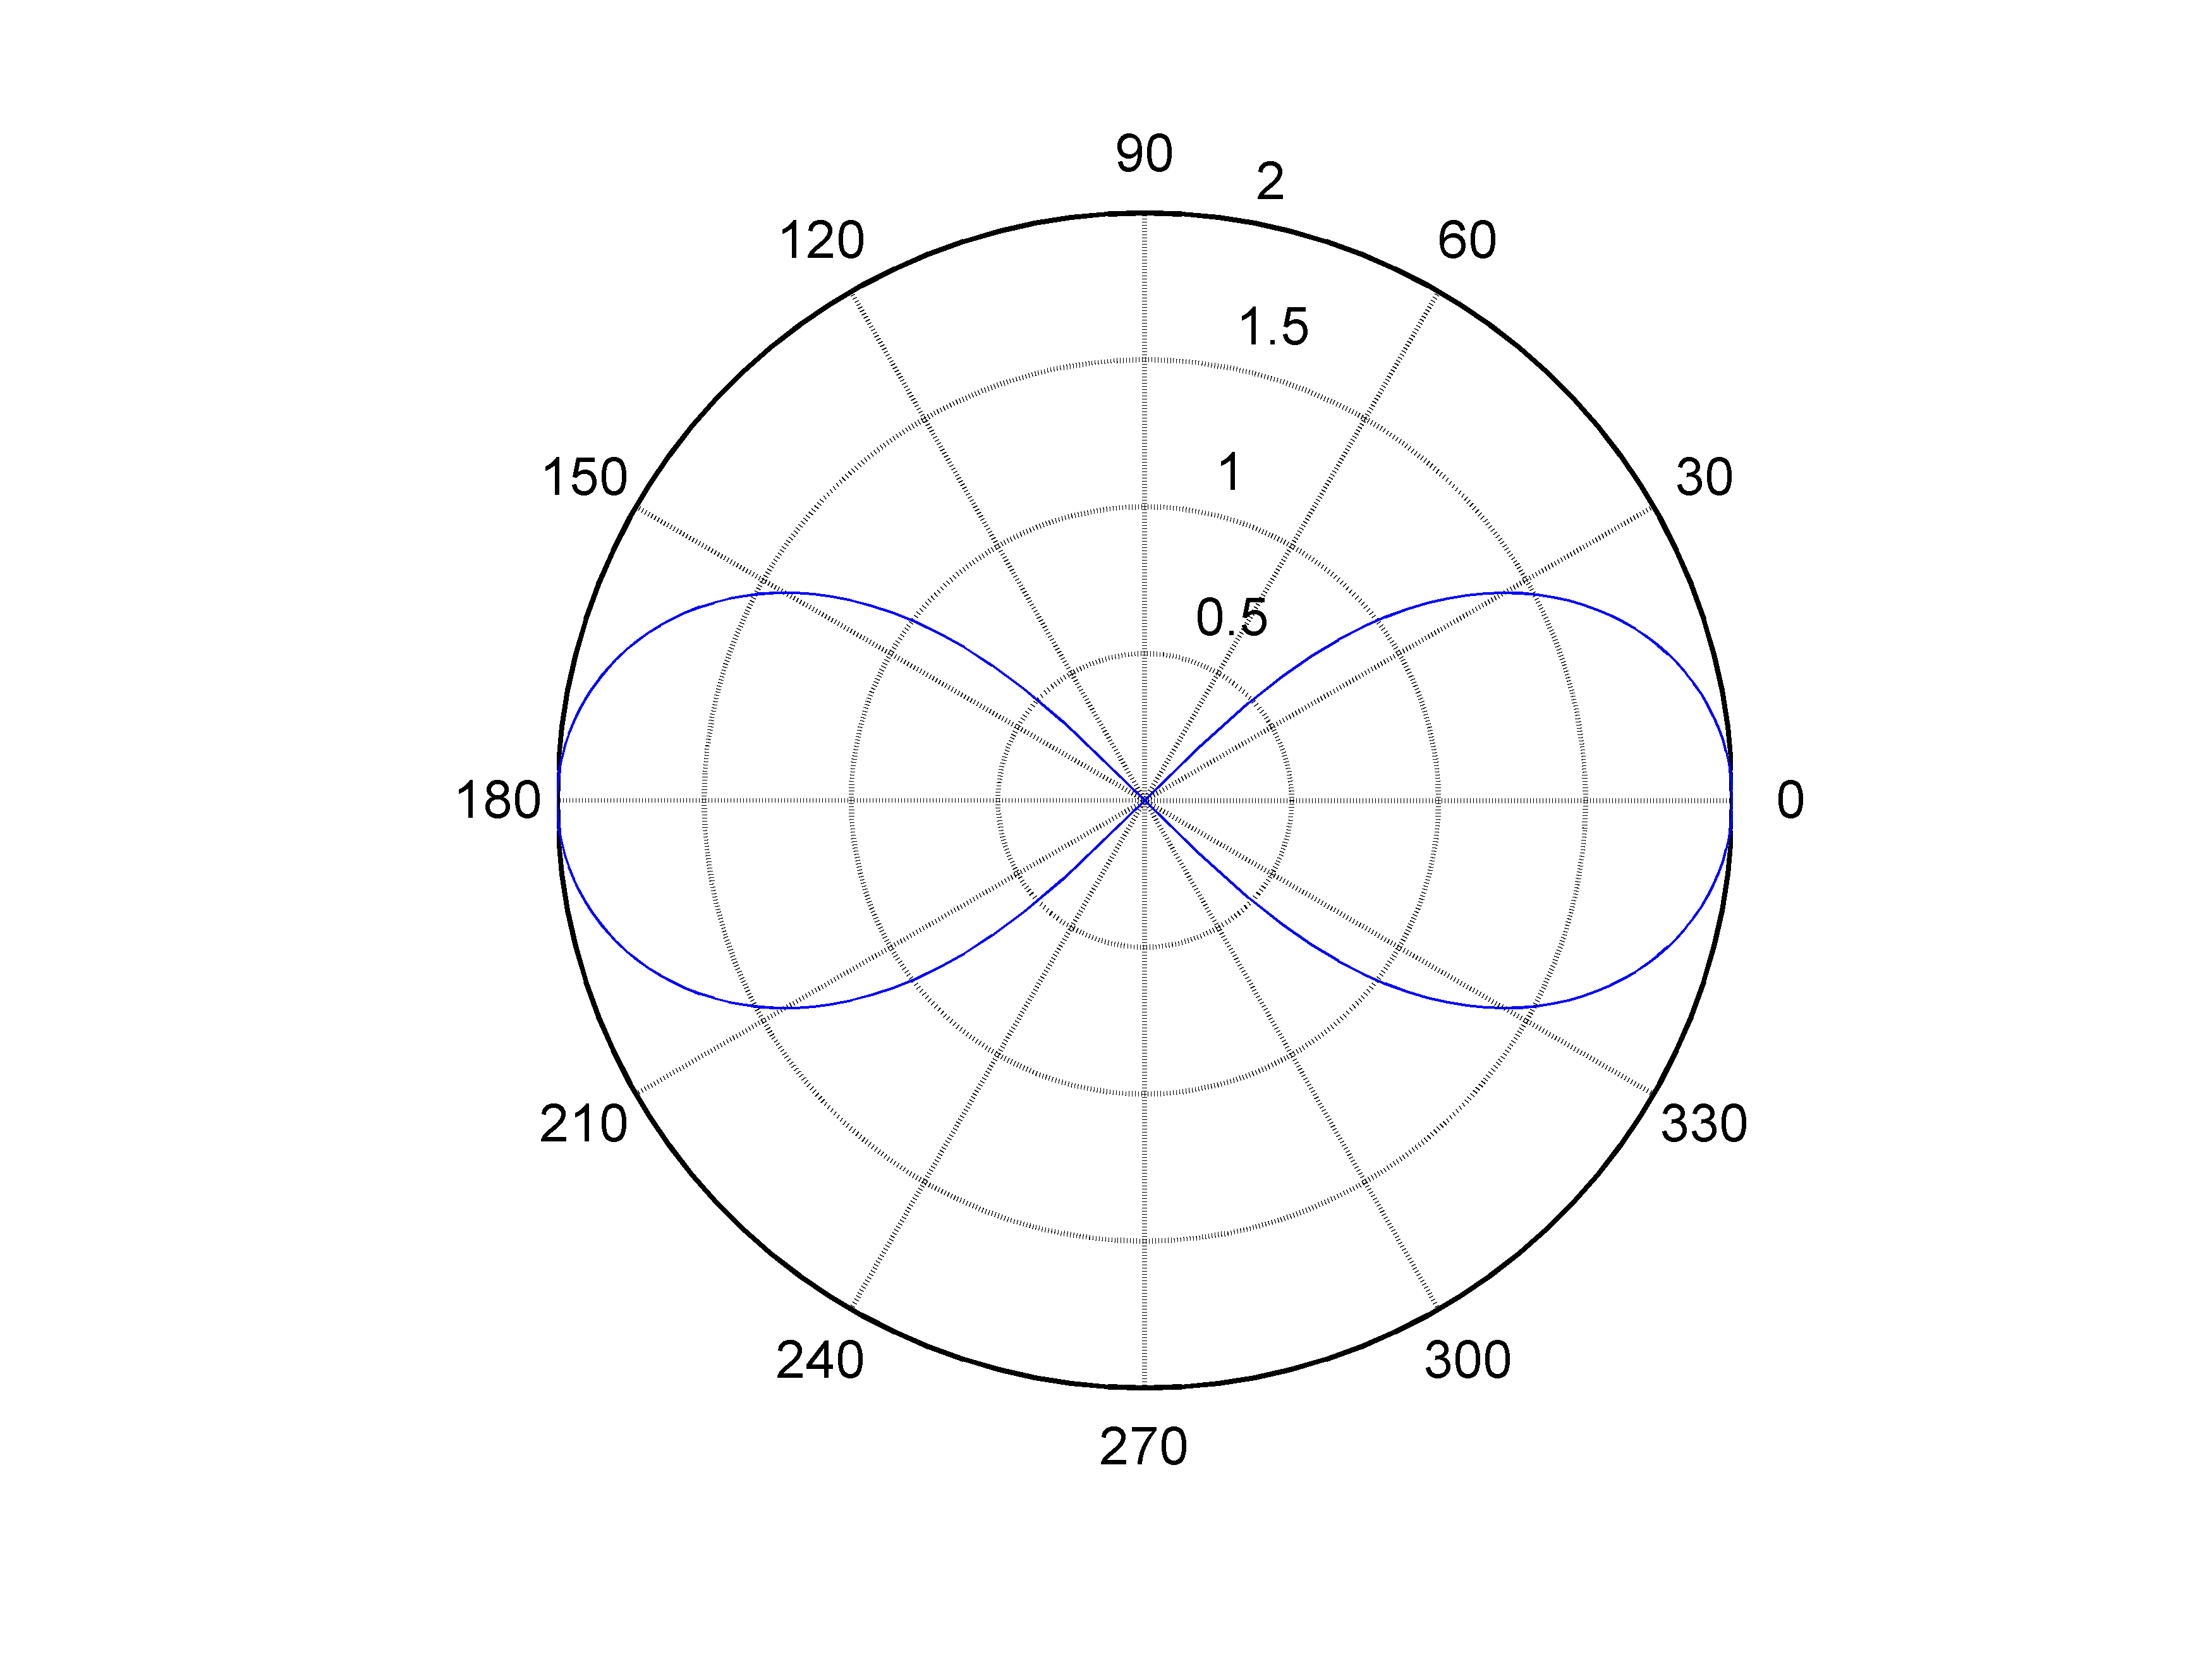
\includegraphics[width=300pt]{./Imagenes/polar2.png}
\end{center} 

\end{enumerate}